%%%%%%%%%%%%%%%%%%%%%%%%%%%%%%%%%%%%%%%%
% datoteka diploma-vzorec.tex
%
% vzorčna datoteka za pisanje diplomskega dela v formatu LaTeX
% na UL Fakulteti za računalništvo in informatiko
%
% vkup spravil Gašper Fijavž, december 2010
% 
%
%
% verzija 12. februar 2014 (besedilo teme, seznam kratic, popravki Gašper Fijavž)
% verzija 10. marec 2014 (redakcijski popravki Zoran Bosnić)
% verzija 11. marec 2014 (redakcijski popravki Gašper Fijavž)
% verzija 15. april 2014 (pdf/a 1b compliance, not really - just claiming, Damjan Cvetan, Gašper Fijavž)
% verzija 23. april 2014 (privzeto cc licenca)
% verzija 16. september 2014 (odmiki strain od roba)
% verzija 28. oktober 2014 (odstranil vpisno številko)
% verija 5. februar 2015 (Literatura v kazalu, online literatura)
% verzija 25. september 2015 (angl. naslov v izjavi o avtorstvu)
% verzija 26. februar 2016 (UL izjava o avtorstvu)
% verzija 16. april 2016 (odstranjena izjava o avtorstvu)
% verzija 5. junij 2016 (Franc Solina dodal vrstice, ki jih je označil s svojim imenom)


\documentclass[a4paper, 12pt]{book}
%\documentclass[a4paper, 12pt, draft]{book}  Nalogo preverite tudi z opcijo draft, ki vam bo pokazala, katere vrstice so predolge!



\usepackage[utf8x]{inputenc}   % omogoča uporabo slovenskih črk kodiranih v formatu UTF-8
\usepackage[slovene,english]{babel}    % naloži, med drugim, slovenske delilne vzorce
\usepackage[pdftex]{graphicx}  % omogoča vlaganje slik različnih formatov
\usepackage{fancyhdr}          % poskrbi, na primer, za glave strani
\usepackage{amssymb}           % dodatni simboli
\usepackage{amsmath}           % eqref, npr.
%\usepackage{hyperxmp}
\usepackage[hyphens]{url}  % dodal Solina
\usepackage{comment}       % dodal Solina

\usepackage[pdftex, colorlinks=true,
						citecolor=black, filecolor=black, 
						linkcolor=black, urlcolor=black,
						pagebackref=false, 
						pdfproducer={LaTeX}, pdfcreator={LaTeX}, hidelinks]{hyperref}

\usepackage{color}       % dodal Solina
\usepackage{soul}       % dodal Solina
\usepackage{listings}	% dodal Hrovat
\usepackage{float}		% dodal Hrovat

%%%%%%%%%%%%%%%%%%%%%%%%%%%%%%%%%%%%%%%%
%	DIPLOMA INFO
%%%%%%%%%%%%%%%%%%%%%%%%%%%%%%%%%%%%%%%%
\newcommand{\ttitle}{Mikrostoritve v decentraliziranem okolju}
\newcommand{\ttitleEn}{Microservices in decentralized environment}
\newcommand{\tsubject}{\ttitle}
\newcommand{\tsubjectEn}{\ttitleEn}
\newcommand{\tauthor}{Primož Hrovat}
\newcommand{\tkeywords}{decentralizacija, distribuirane storitve, tehnologija veriženja podatkovnih blokov}
\newcommand{\tkeywordsEn}{decentralization, distributed services, blockchain}


%%%%%%%%%%%%%%%%%%%%%%%%%%%%%%%%%%%%%%%%
%	HYPERREF SETUP
%%%%%%%%%%%%%%%%%%%%%%%%%%%%%%%%%%%%%%%%
\hypersetup{pdftitle={\ttitle}}
\hypersetup{pdfsubject=\ttitleEn}
\hypersetup{pdfauthor={\tauthor, ph0672@student.uni-lj.si}}
\hypersetup{pdfkeywords=\tkeywordsEn}


 


%%%%%%%%%%%%%%%%%%%%%%%%%%%%%%%%%%%%%%%%
% postavitev strani
%%%%%%%%%%%%%%%%%%%%%%%%%%%%%%%%%%%%%%%%  

\addtolength{\marginparwidth}{-20pt} % robovi za tisk
\addtolength{\oddsidemargin}{40pt}
\addtolength{\evensidemargin}{-40pt}

\renewcommand{\baselinestretch}{1.3} % ustrezen razmik med vrsticami
\setlength{\headheight}{15pt}        % potreben prostor na vrhu
\renewcommand{\chaptermark}[1]%
{\markboth{\MakeUppercase{\thechapter.\ #1}}{}} \renewcommand{\sectionmark}[1]%
{\markright{\MakeUppercase{\thesection.\ #1}}} \renewcommand{\headrulewidth}{0.5pt} \renewcommand{\footrulewidth}{0pt}
\fancyhf{}
\fancyhead[LE,RO]{\sl \thepage} 
%\fancyhead[LO]{\sl \rightmark} \fancyhead[RE]{\sl \leftmark}
\fancyhead[RE]{\sc \tauthor}              % dodal Solina
\fancyhead[LO]{\sc Diplomska naloga}     % dodal Solina


\newcommand{\BibTeX}{{\sc Bib}\TeX}

%%%%%%%%%%%%%%%%%%%%%%%%%%%%%%%%%%%%%%%%
% naslovi
%%%%%%%%%%%%%%%%%%%%%%%%%%%%%%%%%%%%%%%%  


\newcommand{\autfont}{\Large}
\newcommand{\titfont}{\LARGE\bf}
\newcommand{\clearemptydoublepage}{\newpage{\pagestyle{empty}\cleardoublepage}}
\setcounter{tocdepth}{1}	      % globina kazala

%%%%%%%%%%%%%%%%%%%%%%%%%%%%%%%%%%%%%%%%
% konstrukti
%%%%%%%%%%%%%%%%%%%%%%%%%%%%%%%%%%%%%%%%  
\newtheorem{izrek}{Izrek}[chapter]
\newtheorem{trditev}{Trditev}[izrek]
\newenvironment{dokaz}{\emph{Dokaz.}\ }{\hspace{\fill}{$\Box$}}

%%%%%%%%%%%%%%%%%%%%%%%%%%%%%%%%%%%%%%%%%%%%%%%%%%%%%%%%%%%%%%%%%%%%%%%%%%%%%%%
%% PDF-A
%%%%%%%%%%%%%%%%%%%%%%%%%%%%%%%%%%%%%%%%%%%%%%%%%%%%%%%%%%%%%%%%%%%%%%%%%%%%%%%


%%%%%%%%%%%%%%%%%%%%%%%%%%%%%%%%%%%%%%%% 
% define medatata
%%%%%%%%%%%%%%%%%%%%%%%%%%%%%%%%%%%%%%%% 
\def\Title{\ttitle}
\def\Author{\tauthor, ph0672@student.uni-lj.si}
\def\Subject{\ttitleEn}
\def\Keywords{\tkeywordsEn}

%%%%%%%%%%%%%%%%%%%%%%%%%%%%%%%%%%%%%%%% 
% \convertDate converts D:20080419103507+02'00' to 2008-04-19T10:35:07+02:00
%%%%%%%%%%%%%%%%%%%%%%%%%%%%%%%%%%%%%%%% 
\def\convertDate{%
    \getYear
}

{\catcode`\D=12
 \gdef\getYear D:#1#2#3#4{\edef\xYear{#1#2#3#4}\getMonth}
}
\def\getMonth#1#2{\edef\xMonth{#1#2}\getDay}
\def\getDay#1#2{\edef\xDay{#1#2}\getHour}
\def\getHour#1#2{\edef\xHour{#1#2}\getMin}
\def\getMin#1#2{\edef\xMin{#1#2}\getSec}
\def\getSec#1#2{\edef\xSec{#1#2}\getTZh}
\def\getTZh +#1#2{\edef\xTZh{#1#2}\getTZm}
\def\getTZm '#1#2'{%
    \edef\xTZm{#1#2}%
    \edef\convDate{\xYear-\xMonth-\xDay T\xHour:\xMin:\xSec+\xTZh:\xTZm}%
}

\expandafter\convertDate\pdfcreationdate 

%%%%%%%%%%%%%%%%%%%%%%%%%%%%%%%%%%%%%%%%
% get pdftex version string
%%%%%%%%%%%%%%%%%%%%%%%%%%%%%%%%%%%%%%%% 
\newcount\countA
\countA=\pdftexversion
\advance \countA by -100
\def\pdftexVersionStr{pdfTeX-1.\the\countA.\pdftexrevision}


%%%%%%%%%%%%%%%%%%%%%%%%%%%%%%%%%%%%%%%%
% XMP data
%%%%%%%%%%%%%%%%%%%%%%%%%%%%%%%%%%%%%%%%  
\usepackage{xmpincl}
\includexmp{pdfa-1b}

%%%%%%%%%%%%%%%%%%%%%%%%%%%%%%%%%%%%%%%%
% pdfInfo
%%%%%%%%%%%%%%%%%%%%%%%%%%%%%%%%%%%%%%%%  
\pdfinfo{%
    /Title    (\ttitle)
    /Author   (\tauthor, damjan@cvetan.si)
    /Subject  (\ttitleEn)
    /Keywords (\tkeywordsEn)
    /ModDate  (\pdfcreationdate)
    /Trapped  /False
}


%%%%%%%%%%%%%%%%%%%%%%%%%%%%%%%%%%%%%%%%%%%%%%%%%%%%%%%%%%%%%%%%%%%%%%%%%%%%%%%
%%%%%%%%%%%%%%%%%%%%%%%%%%%%%%%%%%%%%%%%%%%%%%%%%%%%%%%%%%%%%%%%%%%%%%%%%%%%%%%

\begin{document}
\selectlanguage{slovene}
\frontmatter
\setcounter{page}{1} %
\renewcommand{\thepage}{}       % preprecimo težave s številkami strani v kazalu
\newcommand{\sn}[1]{"`#1"'}                    % dodal Solina (slovenski narekovaji)

%%%%%%%%%%%%%%%%%%%%%%%%%%%%%%%%%%%%%%%%
%naslovnica
 \thispagestyle{empty}%
   \begin{center}
    {\large\sc Univerza v Ljubljani\\%
      Fakulteta za računalništvo in informatiko}%
    \vskip 10em%
    {\autfont \tauthor\par}%
    {\titfont \ttitle \par}%
    {\vskip 3em \textsc{DIPLOMSKO DELO\\[5mm]         % dodal Solina za ostale študijske programe
%    VISOKOŠOLSKI STROKOVNI ŠTUDIJSKI PROGRAM\\ PRVE STOPNJE\\ RAČUNALNIŠTVO IN INFORMATIKA}\par}%
    UNIVERZITETNI  ŠTUDIJSKI PROGRAM\\ PRVE STOPNJE\\ RAČUNALNIŠTVO IN INFORMATIKA}\par}%
%    INTERDISCIPLINARNI UNIVERZITETNI\\ ŠTUDIJSKI PROGRAM PRVE STOPNJE\\ RAČUNALNIŠTVO IN MATEMATIKA}\par}%
%    INTERDISCIPLINARNI UNIVERZITETNI\\ ŠTUDIJSKI PROGRAM PRVE STOPNJE\\ UPRAVNA INFORMATIKA}\par}%
%    INTERDISCIPLINARNI UNIVERZITETNI\\ ŠTUDIJSKI PROGRAM PRVE STOPNJE\\ MULTIMEDIJA}\par}%
    \vfill\null%
    {\large \textsc{Mentor}: prof.  dr.  Matjaž Branko Jurič\par}%
  % {\large \textsc{Somentor}:  izr.\ prof.\ dr. Martin Krpan \par}%
    {\vskip 2em \large Ljubljana, 2018 \par}%
\end{center}
% prazna stran
%\clearemptydoublepage      % dodal Solina (izjava o licencah itd. se izpiše na hrbtni strani naslovnice)

%%%%%%%%%%%%%%%%%%%%%%%%%%%%%%%%%%%%%%%%
%copyright stran
\thispagestyle{empty}
\vspace*{8cm}

\noindent
{\sc Copyright}. 
Rezultati diplomske naloge so intelektualna lastnina avtorja in Fakultete za računalništvo in informatiko Univerze v Ljubljani.
Za objavo in koriščenje rezultatov diplomske naloge je potrebno pisno privoljenje avtorja, Fakultete za računalništvo in informatiko ter mentorja.

\begin{center}
\mbox{}\vfill
\emph{Besedilo je oblikovano z urejevalnikom besedil \LaTeX.}
\end{center}
% prazna stran
\clearemptydoublepage

%%%%%%%%%%%%%%%%%%%%%%%%%%%%%%%%%%%%%%%%
% stran 3 med uvodnimi listi
\thispagestyle{empty}
\vspace*{4cm}

\noindent
Fakulteta za računalništvo in informatiko izdaja naslednjo nalogo:
\medskip
\begin{tabbing}
\hspace{32mm}\= \hspace{6cm} \= \kill




Tematika naloge:
\end{tabbing}
Besedilo teme diplomskega dela študent prepiše iz študijskega informacijskega sistema, kamor ga je vnesel mentor. V nekaj stavkih bo opisal, kaj pričakuje od kandidatovega diplomskega dela. Kaj so cilji, kakšne metode uporabiti, morda bo zapisal tudi ključno literaturo.

\textbf{TODO:} dopolni z opisom, ko bo na voljo
\vspace{15mm}



\vspace{2cm}

% prazna stran
\clearemptydoublepage

% zahvala
\thispagestyle{empty}\mbox{}\vfill\null\it%
\noindent
Zahvaljujem se prof. Matjažu B. Juriču za podporo in usmeritve pri pripravi diplomskega dela. Posebna zahvala gre mojim staršem, bratom, sestram, starim staršem in prijateljem, ki mi vedno stojijo ob strani in me pri mojem delu podpirajo.
\rm\normalfont

% prazna stran
\clearemptydoublepage

%%%%%%%%%%%%%%%%%%%%%%%%%%%%%%%%%%%%%%%%
% posvetilo, če sama zahvala ne zadošča :-)
% \thispagestyle{empty}\mbox{}{\vskip0.20\textheight}\mbox{}\hfill\begin{minipage}{0.55\textwidth}%
% Posvetilo
% \normalfont\end{minipage}

% prazna stran
\clearemptydoublepage


%%%%%%%%%%%%%%%%%%%%%%%%%%%%%%%%%%%%%%%%
% kazalo
\pagestyle{empty}
\def\thepage{}% preprecimo tezave s stevilkami strani v kazalu
\tableofcontents{}


% prazna stran
\clearemptydoublepage

%%%%%%%%%%%%%%%%%%%%%%%%%%%%%%%%%%%%%%%%
% seznam kratic

\chapter*{Seznam uporabljenih kratic}  % spremenil Solina, da predolge vrstice ne gredo preko desnega roba

\begin{comment}
\begin{tabular}{l|l|l}
  {\bf kratica} & {\bf angleško} & {\bf slovensko} \\ \hline
  % after \\: \hline or \cline{col1-col2} \cline{col3-col4} ...
  {\bf CA} & classification accuracy & klasifikacijska točnost \\
  {\bf DBMS} & database management system & sistem za upravljanje podatkovnih baz \\
  {\bf SVM} & support vector machine & metoda podpornih vektorjev \\
\end{tabular}
\end{comment}

\noindent\begin{tabular}{p{0.1\textwidth}|p{.4\textwidth}|p{.4\textwidth}}    % po potrebi razširi prvo kolono tabele na račun drugih dveh!
  {\bf kratica} & {\bf angleško}                             & {\bf slovensko} \\ \hline
  {\bf API}      & application programming interface & aplikacijski programski vmesnik \\
  {\bf PoW} & Proof-of-Work & Dokaz o opravljenem delu \\
  {\bf DBMS}   & Database Management System & Sistem za upravljanje podatkovne baze \\
  {\bf IPFS} & Interplanetary File System & Medplanetarni datotečni sistem \\
  {\bf REST} & Representational state transfer & - \\
  {\bf GKE} & Google Kontainer Engine & - \\
  {\bf AWS} & Amazon Web Services & - \\
  {\bf DOS} & Denial of Service & Zavrnitev storitve \\
  {\bf CNCF} & Cloud Native Computing Foundation & - \\
\end{tabular}


% prazna stran
\clearemptydoublepage

%%%%%%%%%%%%%%%%%%%%%%%%%%%%%%%%%%%%%%%%
% povzetek
\addcontentsline{toc}{chapter}{Povzetek}
\chapter*{Povzetek}

\noindent\textbf{Naslov:} \ttitle
\bigskip

\noindent\textbf{Avtor:} \tauthor
\bigskip

%\noindent\textbf{Povzetek:} 
\noindent

Mikrostoritve danes počasi a vztrajno prevzemajo primat v svetu razvoja programske opreme.
Nadomeščajo tradicionalne aplikacije, za čim učinkovitejše izvajanje pa obstaja vrsto orodij in tehnik, ki procese skaliranja, distribuiranja in odkrivanja rešujejo na učinkovite načine.
Aplikacije, grajene v arhitekturi mikrostoritev se večinoma izvajajo v velikih računskih centrih - računalniških oblakih.
Vsi ti mehanizmi omogočajo, da smo zmožni odgovoriti na tisoče hkratnih zahtevkov, pri tem pa ohranjamo dobre performančne lastnosti.
Problemi nastopijo ob izpadu enega ali več računskih centrov, oziroma pri prenosu aplikacije iz enega v drug oblačni sistem.
V diplomski nalogi sem raziskal tehnologijo veriženja podatkovnih blokov, ki predstavlja korak v smeri decentralizirane shrambe podatkov.
Podobno stopnjo decentralizacije želimo doseči na ravni aplikacijske logike in sicer na način, kjer bi poljubno storitev lahko izvajal poljuben član omrežja, za uspešno izvajanje pa bil tudi primerno finančno nagrajen.
Zamišljamo si sistem, v katerem ne poznamo izpadov storitev ter dolgih odzivnih časov.
Sistem decentraliziranega izvajanja bi nam hkrati olajšal finančno evaluirati posamezen klic, ter omogočil učinkovito izmenjavo vrednosti.
V nalogi sem se predvsem na decentralizirano odkrivanje storitev, ter razvil prvi prototip aplikacije ter razširitve za ogrodje KumuluzEE, ki demonstrirata decentraliziran način izvajanja.
Gre za pomembno svetovno novost, ki ima potencial začrtati nove smernice v računalniški panogi.
Stojimo na robu znanih mej, ki jih želimo potisniti dalje.

\bigskip

\noindent\textbf{Ključne besede:} \tkeywords.
% prazna stran
\clearemptydoublepage

%%%%%%%%%%%%%%%%%%%%%%%%%%%%%%%%%%%%%%%%
% abstract
\selectlanguage{english}
\addcontentsline{toc}{chapter}{Abstract}
\chapter*{Abstract}

\noindent\textbf{Title:} \ttitleEn
\bigskip

\noindent\textbf{Author:} \tauthor
\bigskip

%\noindent\textbf{Abstract:} 
\noindent 

Microservices today are one of the leading design principles, when it comes to building modern applications.
Monoliths are being replaced with this modern architecural style and multiple tools and techniques are being develop to support it.
Applications are deployed to a remote computing center, often called simply as cloud.
These principles allow us to effectively respond to thousands requests per second.
The problems arrise when those cloud providers experience massive breakdowns or we wish to commute to different cloud provider.
My thesis discusses blockchain technology that is currently one of the hot research topics.
Blockchain provides decentralized and immutable data storage.
Our vision is to enable that kind of decentralization to bussines logic (API) in a way that everyone can participate, either by executing any of available services or consuming it.
Executors are rewarded financially and the system enables us to efficiently transfer value.
To achive that goal, we must solve multiple problems, one of which is decentralized service discovery.
I have proposed a conceptual solution to service discovery in a decentralized environment and implemented first prototype, that enables decentralized execution of applications.
We are standing on the edge of what we know is currently possible and are ready to push the boundaries even further. This can be the next big step in computer science.

\bigskip

\noindent\textbf{Keywords:} \tkeywordsEn.
\selectlanguage{slovene}
% prazna stran
\clearemptydoublepage

%%%%%%%%%%%%%%%%%%%%%%%%%%%%%%%%%%%%%%%%
\mainmatter
\setcounter{page}{1}
\pagestyle{fancy}

\chapter{Uvod}
Poslovne storitve se danes selijo v oblak.
S pojavom arhitekture mikrostoritev in podporne tehnologije, kot so vsebniki in okolja za orkestracijo vsebnikov, so, nekdaj ogromni, kosi programske opreme pričeli razpadati na manjše, logično ločene sestavne dele.
Razmeroma majhne in neodvisne aplikacije, specializirane za opravljanje točno določenih nalog, omogočajo hiter vzpostavitveni čas in puščajo majhen odtis na porabi strojne opreme.
Neodvisnost teh aplikacij nam omogoča tudi skaliranje teh posamenznih delov celotne storitve, ko je to potrebno.
Vsebniki so razmeroma stara tehnologija, ki je s pojavom okolja Docker doživela pravi razcvet.
Gre za \sn{lahko} obliko virtualizacije, virtualizacija tu poteka na nivoju procesov in ne operacijskega sistema.
Pravi potencial vsebnikov izkoristimo šele z uporabo orkestratorjev, kot so Kubernetes, Amazon ECS, Google Container Engine (GKE), Docker Swarm, Azure Container Service in podobni.
Ta orodja omogočajo monitoring, zaganjanje, zaustavljanje in preverjanje storitev, skladno s podanimi zahtevami.
Storitve se izvajajo distribuirano (porazdeljeno) in replicirano, lahko tudi na fizično ločenih sistemih, kar zagotavlja visoko stopnjo odzivnosti in dosegljivosti. Stopnja dosegljivosti se danes meri na peti ali šesti decimalki (\sn{number of nines}).

S pojavom Bitcoina se je začel razvoj tehnologije, ki v decentraliziranem okolju omogoča varno in nespremenljivo hrambo podatkov.
Veriženje podatkovnih blokov je v zadnjih letih s pojavom različnih organizacij kot so Hyperledger in Ethereum doživelo razcvet.
Nova tehnologija omogoča shranjevanje podatkov, repliciranih na vseh sodelujočih entitetah v omrežju, obenem pa zagotavlja njihovo nespremenljivost.

Tu se pojavlja vprašanje. 
Je možno tudi poslovno logiko prestaviti v decentralizirano okolje na način, da bo sodelujoči v omrežju ob klicu želene storitve vedno dobil odgovor, izvedla ga bo katerakoli entiteta, obenem pa zagotoviti pravilnost izvajana?
Z uresničitvijo tega cilja bi miselnost decentraliziranih podatkov prestavili nivo višje, na nivo poslovne logike.
Odzivnost in dosegljivost storitve bi s številom sodelujočih v omrežju dosegla 100\%, prav tako bi bilo praktično nemogoče izvesti napade DOS.
Gre za sistem neodvisnih entitet, ki so pripravljene proti primernemu plačilu, izvajati storitve na željo naročnika.
Vsakdo lahko sodeluje, vsakdo lahko prispeva, vsako uspešno operacijo sistem samodejno nagradi.
Tak sistem sestavlja veliko komponent, vsaka izmed njih potrebuje dobršno mero pozornosti in raziskovalnega dela. Ena izmed osrednjih komponent je način, kako v decentraliziranem okolju odkriti druge, trenutno aktivne storitve, ko jih naša storitev potrebuje. 
V diplomski nalogi sem se podrobneje posvetil reševanju tega problema, pred tem pa je predstavljenih nekaj tehnologij in tehnik, ki so za moje raziskovalno delo relavantne.


\chapter{Arhitekturni koncepti mikrostoritev}
\label{ch1}

Razvoj monolitov je enostaven in danes dobro podprt v vseh danes prisotnih razvojnih okoljih.
Prenos in namestitev teh storitev na strežniške sisteme je enostaven postopek, rešitev v obliki izvršljivih datotek ali s kopiranjem direktorijske strukture prenesemo v produkcijsko izvajalno okolje.
Če želimo tako storitev skalirati, kot vstopno točko v naše zaledne sisteme nastavimo izenačevalnika obremenitev (ang. load balancer), ki poskrbi za enakomerno porazdeljevanje dela med posameznimi instancami storitve.

Slabosti te arhitekture se pojavijo, ko storitev postane kompleksnejša.
Podaljša se zagonski čas (start up time), ob preobremenitvi le enega dela storitve je potrebno instancirati celotno aplikacijo.
Prav tako je otežen proces sprotne dostave (Continouos Delivery) in sprotne integracije (Continouos Integration), za posodobitev enega dela sistema je namreč potrebno celotno storitev zaustaviti, namestiti novo različico in jo ponovno zagnati \cite{monolithMicroservice}.


\section{Arhitektura mikrostoritev}

Gradnja aplikacij je do nedavnega potekala na način, da so razvijalci vse odvisnosti in logiko, potrebno za delovanje, zložili skupaj v veliko tvorbo - monolit.
Tak način gradnje ima svoje prednosti in slabosti.
Prednosti na eni strani predstavljajo enostavna zgradba aplikacije, ker je vsa izvorna koda zbrana na enem mestu.
Orodja za razvoj so prilagojena takemu načinu dela in razvijalcu ponujajo širok nabor funkcij, ki podpirajo celotno življenjko pot aplikacije, od razvoja, testiranja, namestitve v testna in produkcijska okolja ter vzdrževanje.
Velikost projekta je na drugi strani ena od slabosti monolitov, majhne spremembe enega sestavnega dela potrebujejo ponovno namestitev celotne aplikacije.
Skaliranje poteka vertikalno, le preko ustvarjanja novih instanc celotne aplikacije.
Monolitna zasnova aplikacije razvijalce in vzdrževalce zaveže k dolgoročni uporabi tehnologij, ki so bile uporabljene na začetku.
Kasnejše uveljavljanje novih tehnologij oziroma nadomeščanje obstoječih je časovno in finančno potratno, saj je potrebno celotno logiko aplikacije prepisovati \cite{monolithMicroservice}.

Arhitektura mikrostoritev se problema gradnje aplikacij loti drugače.
Celotno aplikacijo se logično razbije na posamezne sestavne dele, ki se izvajajo samostojno in se med seboj povezujejo preko lahkih komunikacijskih protokolov.
Vsak sestavni del aplikacije je samostojen v smislu skaliranja, življenjske dobe posamezne instance, razvoja in podpornih tehnologij.
Tak način gradnje sledi tistemu, ki ga v fizičnem svetu poznamo že stoletja, to je sestavljanje vnaprej pripravljenih delov v celoto.
Lep primer tega je avtomobilska industrija.
Na tekočem traku se na tisoče sestavnih delov različnih proizvajalcev zloži v polno funkcionalno enoto - avtomobil.
Podobno želimo doseči pri razvoju programske opreme, kar bi pohitrilo in pocenilo razvoj novih aplikacij, krepko pa bi omejili tudi nepotrebno podvajanje izvorne kode \cite{microservicePattern, microservicesMartin}.

V povezavi z mikrostoritvami je tesno povezana tudi arhitektura \sn{cloud-native}.
Gre za novo paradigmo razvoja programske opreme, ki sledi načinom izdelave stvari v fizičnem svetu.
Z namenom uveljavljanja in razvoja paradigme je bila ustanovljena \sn{Cloud Native Computing Foundation}, ki bdi nad razvojem standardov in novih smernic.
Oblačne sisteme sestavljajo \cite{cncf}:
\begin{itemize}
	\item Aplikacije in procesi, ki se izvajajo znotraj vsebnikov. Vsebniki so neodvisne in izoloirane izvajalne enote.
	\item Storitve, ki se dinamično upravljajo in nadzorujejo preko centralnega orkestracijskega procesa.
	\item Mikrostoritve, ki sos sestavni deli sistema in so med seboj šibko sklopljene.
\end{itemize}

Računalništvo v oblaku je uporaba in dostop do računskih virov (aplikacije, podatkovna skladišča, procesorski čas...) na zahtevo preko interneta.
Plačilo se izvede skladno s količino porabljenih virov.
Viri so elastični in zmožni hitrega in učinkovitega skaliranja ter prilagajanja trenutnim zahtevam.
V grobem med seboj ločimo tri glavne komponente oblačnih sistemov: SaaS, PaaS in IaaS.
SaaS (Software as a Service) - programska oprema kot storitev, je oblačna aplikacija, ki se izvaja na oddaljenih računalnikih, do katerih uporabnik storitve dostopa preko interneta. 
Prednosti teh aplikacij so dostopnost od koderkoli, za nemoteno delovanje aplikacije je odgovoren ponudnik.
Storitev je zmožna dinamičnega skaliranja, da zadovolji trenutnim potrebam.
PaaS (Platform as a Service) - platforma kot storitev, uporabnikom ponuja programsko platformo, brez stroškov nakupa in kompleksnosti upravljanja podporne strojne in programske opreme.
IaaS (Infrastructure as a Service) - infrastruktura kot storitev, ponuja dostop do računskih virov (strežniki, omrežna oprema, shramba...).
Uporabnikom ni potrebno investirati v lastno strojno opremo, podobno kot obe sestrski storitvi (SaaS in PaaS), je tudi ta zmožna samodejnega skaliranja \cite{ibmCloudComputing}.


\section{Vzorci}

Ena funkcionalna enota, šibka sklopljenost.

V tem podpoglavju predstavljam še tri vzorce, značilne za arhitekturo mikrostoritev: metrike, preverjanje odzivnosti ter odkrivanje storitev.
Te tri storitve skupaj predstavljajo skoraj vse elementarne dele sistema za decentralizirano izvajanje.
Za učinkovit sistem potrebujemo načine, kako ugotoviti, katere storitve delujejo po pričakovanjih in katere ne, ter katera izmed sodelujočih entitet v omrežju nam lahko najhitreje ponudi odgovor na zahtevo -- izvede storitev.

\subsection{Metrike}

Posamezna storitev se lahko izvaja na različnih (fizičnih) lokacijah, na različni strojni opremi in v več instancah.
Pojavi se potreba po spremljanju storitve in njenega obnašanja, kje in zakaj prihaja do izpadov oziroma morebitnih dolgih odzivnih časih.
Vse želene metrike želimo shraniti na enem centralnem mestu, jih po možnosti agregirati, in tako omogočiti enostavno odkrivanje napak in njihovo reševanje.
V osnovi poznamo dva modela zbiranja metrik: 
\begin{itemize}
	\item mikrostoritev sama pošilja metrike centralni zbirki (push)
	\item centralna zbirka zahteva metrike od storitve (pull)
\end{itemize}

Zbiranje metrik ponuja dober vpogled v obnašanje posameznih storitev, s sabo pa prinese dodatno potrebno infrastrukturo in dodatne težave pri implementaciji \cite{ApplicationMetrics}.


Ena izmed bolj znanih storitev za zbiranje aplikacijsih metrik je Prometheus, odprtokodna zbirka orodij za zbiranje in agregiranje metrik ter obveščanje.
Projekt je bil, takoj za orkestracijskim okoljem Kubernetes, pridružen fundaciji CNCF.
Prometheus zahteva metrike od storitve (način pull), jih agregira in proži morebitna opozorila.
Skupaj z ogrodjem Grafana omogoča celovit grafičen vpogled v zbrane metrike \cite{Prometheus}.

\subsection{Preverjanje odzivnosti (Health Check)}

Pogosto se zgodi, da se storitev še vedno odziva na posamezne zahteve, vendar so te neuspešne.
V takšnih primerih je pričakovano obnašanje sistema, da nedelujočo storitev iz omrežja označi kot nedosegljivo in jo nadomesti z novo.
Tu v igro vstopi koncept preverjanja odzivnosti storitev (ang. Health check), ki za vsako storitev pričakuje izpostavljeno dostopno točko, preko katere lahko sistem pridobi informacije o sposobnosti storitve, da odgovori na zahtevke.
Vsaka storitev je odgovorna za preverjanje svojih zunanjih in notranjih virov in generiranja poročila o trenutnem statusu posamezne komponente.
Tipični testi so preverjanje zmožnosti povezave na podatkovno bazo, dosegljivost ostalih odvisnih storitev, povezljivost z vrstami...
Poleg zunanjih odvisnosti se preveri tudi stanje gostitelja: razpoložljiv prostor na disku, zasedenost CPE ipd.
Nadzorna storitev periodično proži zahteve na vse registrirane storitve in preverja njihove odzive.
Tipičen ukrep ob negativnem odzivu je zaustavitev in ponovni zagon nedelujoče storitve \cite{healthCheck}.

\subsection{Odkrivanje storitev (Service discovery)}

Ko želimo od zunanje entitete pridobiti podatke oziroma prožiti določeno akcijo, potrebujemo njen omrežni naslov (kombinacija naslova IP in številke vrat).
Pri klasičnih aplikacijah, ki se izvajajo na fizični napravi, so naslovi relativno statični.
Zelo malo je tudi klicev med posameznimi aplikacijami, saj se storitve med seboj kličejo preko programskih klicev.
V arhitekturi mikrostoritev je omrežnih klicev bistveno več, ker je celotna programska logika aplikacije sestavljena iz več samostojnih storitev.
Njihovo število se dinamično spreminja, skladno s tem tudi omrežni naslovi posameznih instanc.
Posledično je potrebno za odjemalca vpeljati nov mehanizem, ki je zmožen dinamično odkriti naslove, na katerih se želena storitev nahaja.

Tipično za oblačne arhitekture je, da se odkrivanje storitev realizira s pomočjo centralnega registra.
Storitve se ob pričetku izvajanja registrirajo.
Odjemalska aplikacija ob potrebi po dostopu do zunanje storitve na register naslovi poizvedbo za lokacijo instanc želene mikrostoritve.
Zakasnitev pri omrežnih klicih je bistveno večja kot pri programskih klicih znotraj aplikacije, zato želimo visoko učinkovitost poizvedb \cite{serviceDiscovery, maldip}.

\section{Vsebniki in orkestracija}

Vsebniki danes nadomeščajo virtualne naprave, predvsem na račun bolj učinkovite uporabe sistemskih virov in odpravljanjem nepotrebnih podvajanj programske opreme.

\subsection{Tehnologija vsebnikov}
Vsebnik je samostojen, izvršljiv skupek programske opreme, ki vsebuje vse potrebne odvisnosti, orodja, knjižnice in nastavitve, potrebne za izvajanje.
Izvajanje kode znotraj vsebnika bo v vsakem gostiteljskem ogrodju (Windows, Linux, MacOS) enako.
Notranji deli vsebnika so izolirani od okolice, kar odpravlja morebitne konflikte zaradi različnih verzij potrebnih odvisnosti.
V primerjavi z navideznimi napravami, vsebniki virtualizirajo operacijski sistem in ne podporne strojne opreme.
Z gostiteljskim sistemom in ostalimi vsebniki delijo jedro operacijskega sistema, vsak izmed njih v svojem naslovnem prostoru.

Shema \ref{vm_vs_container} prikazuje bistveno razliko med vsebniško tehnologijo in tehnologijo virtualizacije \cite{dockerContainer}.

\begin{figure}[h]
	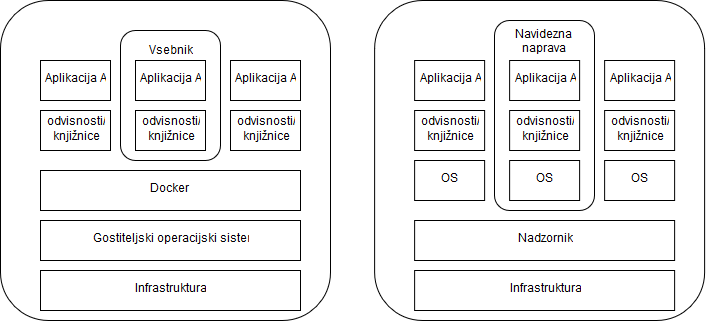
\includegraphics[width=1.0\textwidth]{slike/vsebniki_vm.png}
	\label{vm_vs_container}
	\caption{Primerjava vsebnikov in navideznih naprav}
\end{figure}


\subsection{Orkestracijska orodja}

Proces prenosa in namestitve vsebnikov v izvajalno okolje je moč avtomatizirati.
Proces postaja pomembnejši z rastjo števila vsebnikov in gostiteljskih sistemov. 
Ta tip avtomatizacije imenujemo orkestracija, ponuja pa nam vrsto funckionalnosti \cite{mongoKubernetes}:
\begin{itemize}
	\item upravljanje z gostiteljskim sistemom
	\item instanciranje vsebnikov
	\item upravljanje z vsebniki
	\item povezovanje vsebnikov preko vmesnikov
	\item izpostavljanje storitev zunanjim napravam
	\item skaliranje gruče vsebnikov
\end{itemize}

S pojavom in razširitvijo vsebniške tehnologije so se pojavila tudi številna orodja za orkestracijo.
Med njimi najbolj poznana sta Docker Swarm in Kubernetes.
Vsako izmed teh orodij orkestracijo rešuje na svoj način, Kubernetes pa je trenutno eno izmed najbolj razširjenih orodij.
Njegove glavne funckionalnosti so:
\begin{itemize}
	\item avtomatizirano nameščanje in repliciranje vsebnikov
	\item skaliranje
	\item porazdeljevanje dela (load balancing)
	\item nameščanje posodobitev
	\item odpornost na napake in odpovedi vsebnikov z avtomatskimi ponovnimi zagoni
	\item kontrolirano izpostavljanje notranjega omrežja zunanjim storitvam
\end{itemize}

Glavni sestavni deli Kubernetesa \cite{mongoKubernetes}: 
\begin{itemize}
	\item gruča: zbirka enega ali več strežnikov (ang. Node), ki svoje vire ponujajo nadzornemu procesu
	\item strok (pod): skupina vsebnikov in pripradajočih shramb, ki so dodeljene enemu gostitelju. Predstavljajo osnovno celico Kubernetesa, znotraj stroka si procesi delijo lokalni omrežni naslovni prostor.
	\item labele: dodeljene oznake posameznim entitetam (vsebnikom), ki omogočajo upravljanje z njimi v skupini
	\item storitve: skrbijo za osnovno dodeljevanje dela in izpostavljajo stroke zunanjemu svetu.
\end{itemize}

Slika \ref{kubernetes_cluster} prikazuje osnovno shemo Kubernetes gruče.

\begin{figure}[h]
	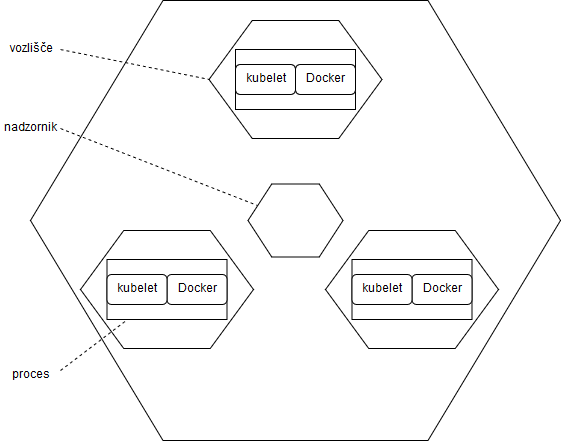
\includegraphics[width=1.0\textwidth]{slike/kubernetes_cluster.png}
	\label{kubernetes_cluster}
	\caption{Kubernetes gruča \cite{kubernetesTutorial}}
\end{figure}


\chapter{Tehnologija veriženja podatkovnih blokov}
\label{ch2}

Izvajanje poslovne logike aplikacije uvrščamo med nivo hrambe podatkov in nivojem uporabniškega vmesnika.
Decentralizirano hrambo podatkov danes že poznamo, od tu pa gradimo in razmišljamo naprej, v smeri decentralizacije poslovne logike.
V tem poglavju bom predstavil tehnologijo in osnovne ideje, ki omogočajo porazdeljeno hrambo podatkov.
Koncepti, ki so tu v uporabi, predstavljajo osnovo in odskočno desko za decentralizacijo izvajanja storitev.
Podatkovni bloki nam omogočajo trajno in nespremenljivo sklepanje ter zapis dogovorov o podrobnostih izvajanja, kar je nujno za zanesljiv sistem takšnih storitev.

Veriženje podatkovnih blokov je peer-to-peer porazdeljena podatkovna shramba, dosežena s soglasjem, sistemom \sn{pametnih} pogodb ter drugih pomožnih tehnologij \cite{hyperledgerWeb}. Osrednja komponenta sistema je glavna knjiga (ang. ledger), ki beleži vse akcije (transakcije), izvedene na omrežju \cite{hyperledgerDocs}.
Entiteta, ki transakcijo izvede, jo podpiše s svojim privatnim ključem.
Skupek transakcij tvori podatkovni blok, bloki pa se med seboj povezujejo v podatkovno verigo.
Posamezne člene verige med seboj povezuje zgoščevalna funkcija, na vhod katere postavimo zgoščeno vrednost trenutnega in prejšnjega bloka.
Podatkovno verigo je moč vedno le podaljševati, trenutno veljavno in resnično stanje omrežja je trenutno najdaljša serija blokov.
Celotna veriga blokov je replicirana na vsaki izmed sodelujočih entiteti.

Kombinacija teh pristopov omogoča, da nobena izmed sodelujočih entitet ne more spreminjati že zapisanih blokov.
Napad na omrežje je možen le s pridobitvijo več kot polovice vseh sodelujočih entitet v omrežju, ki bi potrjevale resničnost ponarejenih transakcij in sčasoma sestavile daljšo podatkovno verigo, ki bi obveljala kot trenutna resnica.
S temi mehanizmi se zagotovi veljavnost in nespremenljivost podatkov v okolju, ki mu apriori ni potrebno zaupati.
Ni več potrebe po zunanji, zaupanja vredni, entiteti.

Za interakcijo z glavno knjigo in zapisovanje novih informacij, omrežje uporablja t.i. \sn{pametne pogodbe}.
To je del programske kode, ki se lahko odziva na dogodke v omrežju, izvede zapisano poslovno logiko ter ustvarja nove transakcije \cite{hyperledgerDocs}.

V nadaljevanju tega poglavja se bom posvetil osnovnim konceptom ter predstavil posebnosti dveh implementacij te tehnologije - omrežji Ethereum in Hyperledger Fabric.
Osredotočil sem se predvsem na ti dve, ker do rešitve problema pristopata z različnih koncev.
Prva predpostavlja popolnoma javno omrežje, kjer so identitete uporabnikov neznane, druga svoje prednosti gradi na predpostavki popolnega zaupanja med sodelujočimi identitetami.
V želji zgraditi sistem, ki bo omogočal decentralizirano izvajanje storitev in preprečeval morebitne poneverbe izvedbe posameznih operacij, hkrati pa zagotavljal popolnoma anonimnost udeležencev, je verjetno smiselno uporabiti nekakšno fuzijo obeh pristopov.

\section{Razlaga osnovnih konceptov}

\subsection{Porazdeljena glavna knjiga}
V osrčju tehnologije podatkovnih blokov je porazdljena glavna knjiga, ki vsebuje zapise o vseh transakcijah, izvedenih na omrežju.
Glavna knjiga je replicirana na vseh entitetah v omrežju, ki med sabo sodelujejo in skrbijo za vzdrževanje.
Informacije so v glavno knjigo le dodajajo z uporabo kriptografskih tehnik, ki zagotavljajo, da je vsaka zapisana transakcija trajna in nespremenljiva.
To omogoča enostavno preverjanje izvora informacije, od tu tudi drugo poimenovanje za tehnologijo podatkovnih blokov kot sistem dokazovanja \cite{hyperledgerDocs}.
Na sliki \ref{hyperledger_basic_network} je prikazana osnovna shema omrežja.

\begin{figure}[h]
	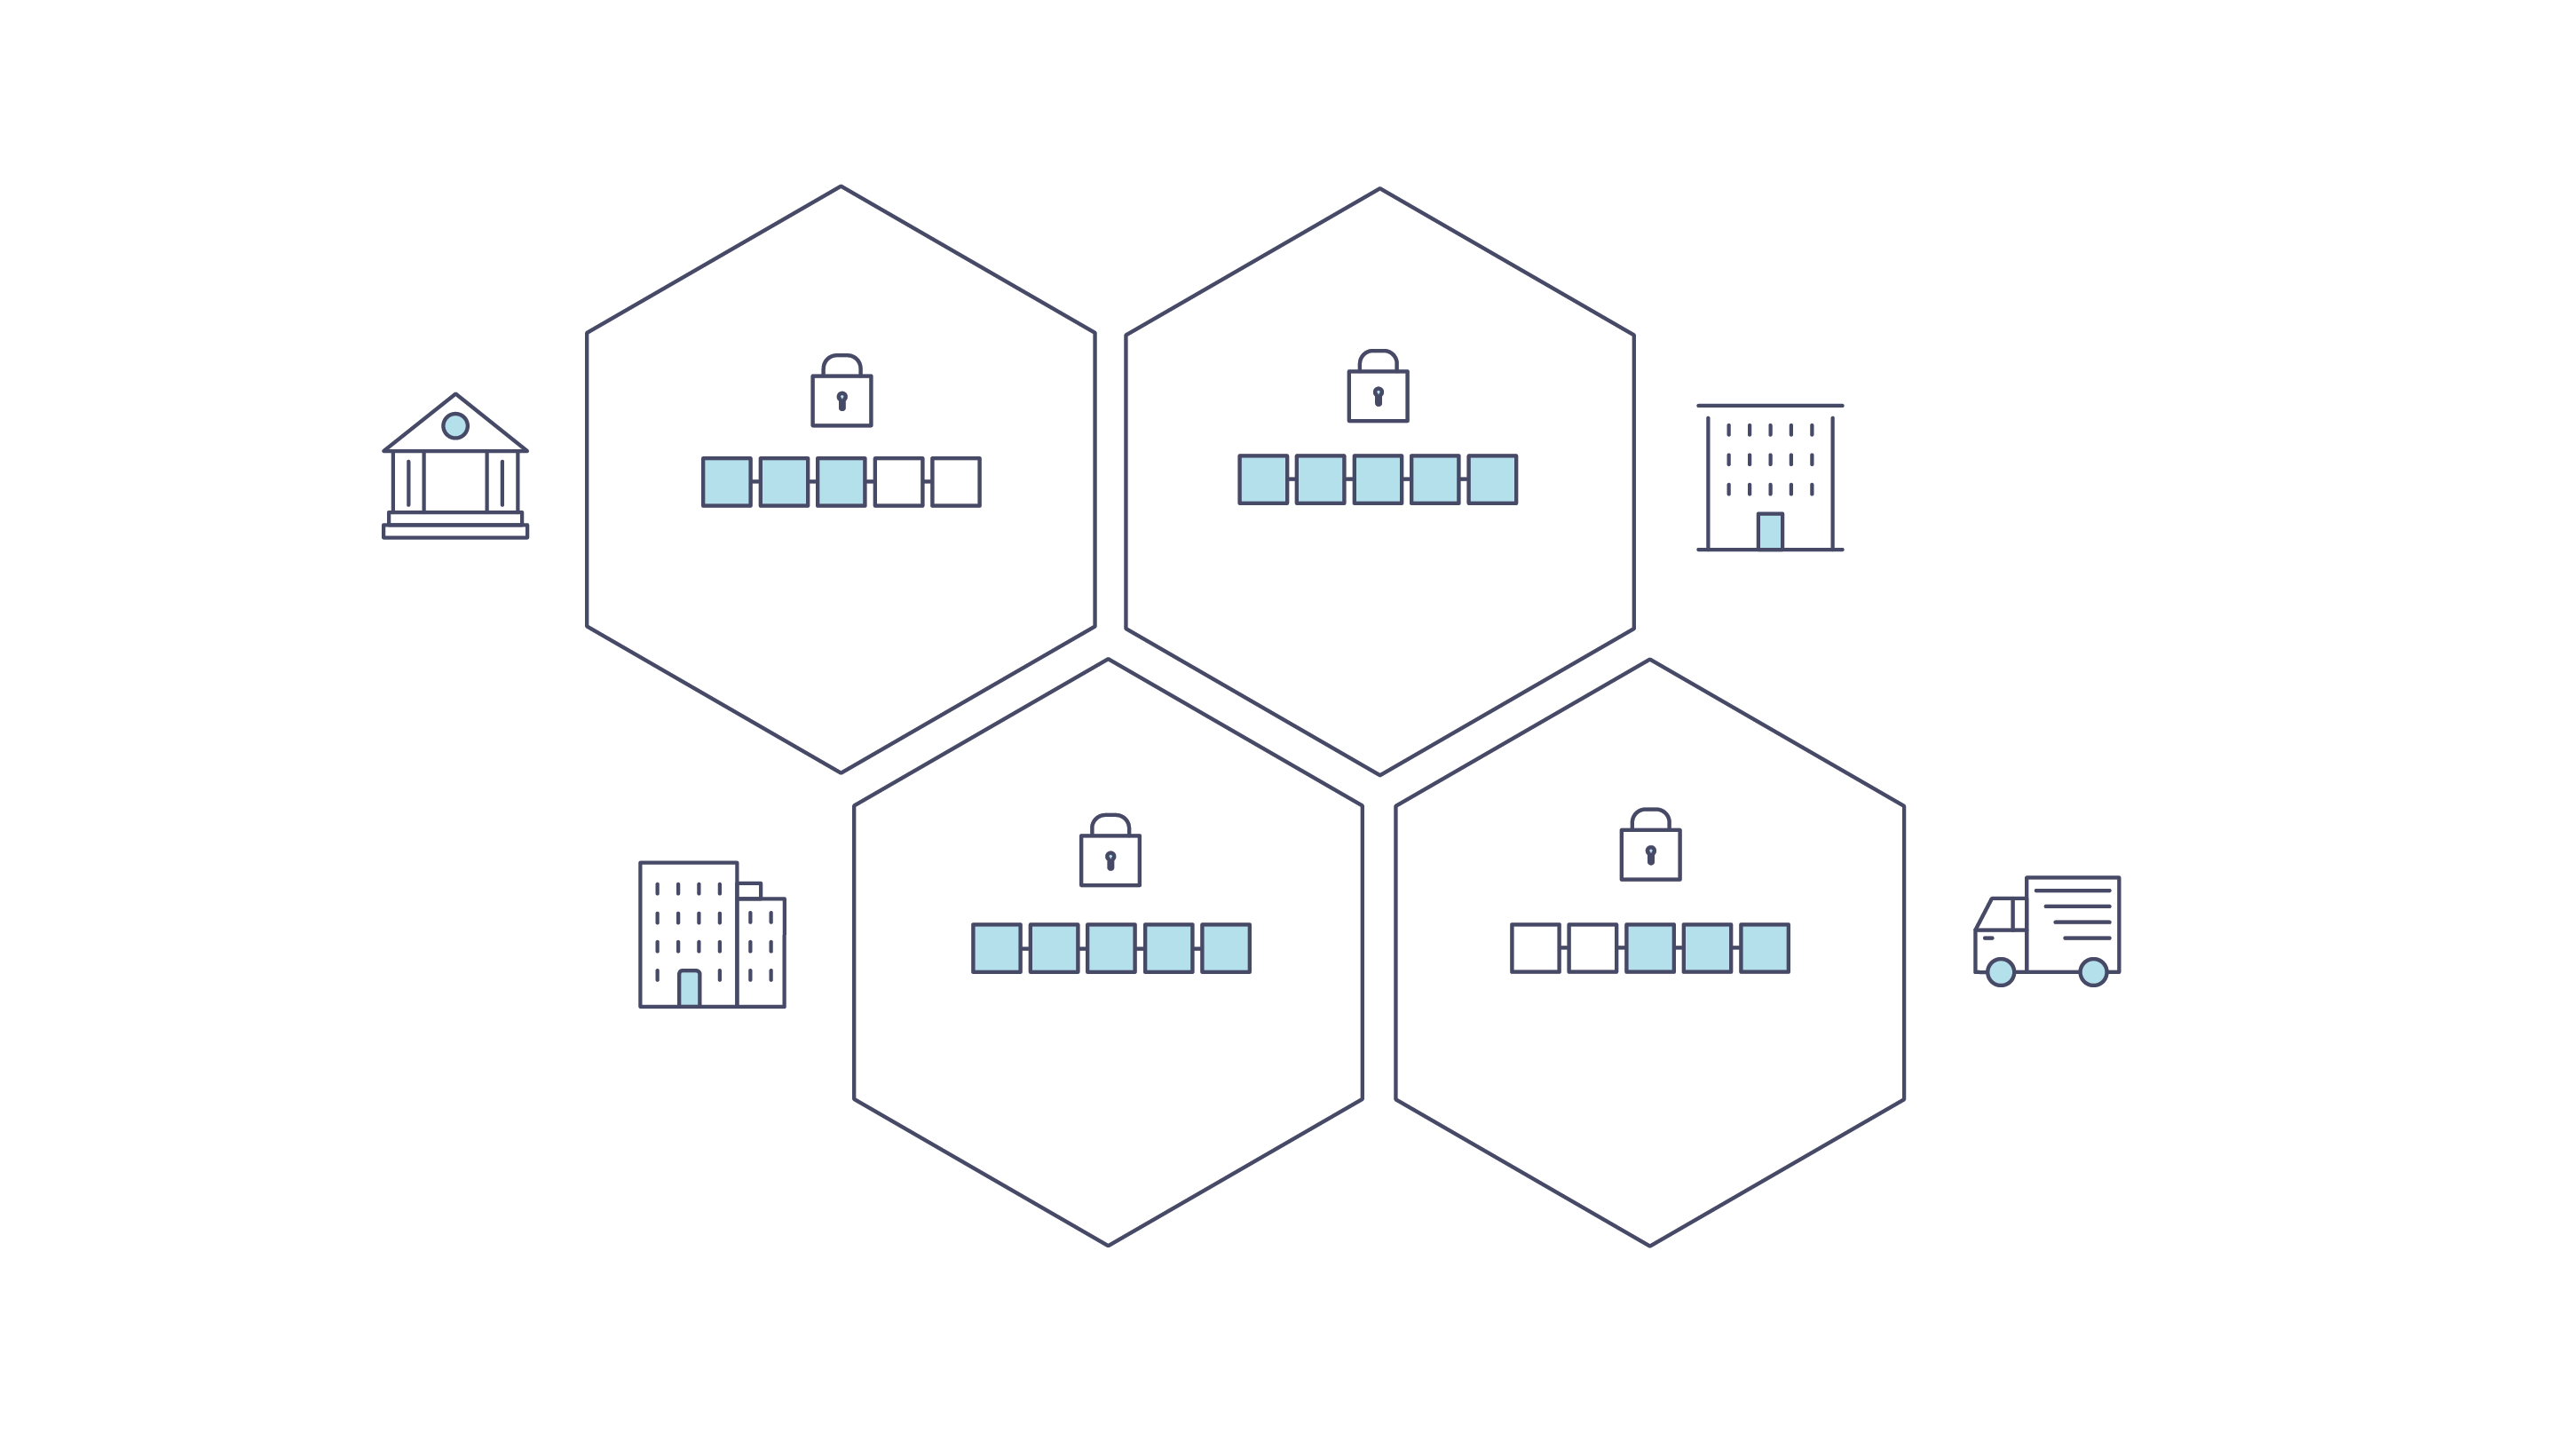
\includegraphics[width=1.0\textwidth]{slike/basic_network.png}
	\label{hyperledger_basic_network}
	\caption{Porazdeljeno omrežje. Vsak uporabnik hrani kopijo glavne knjige \cite{hyperledgerDocs}}.
\end{figure}

\subsection{Pametne pogodbe}
Pametne pogodbe omogočajo kontroliran dostop in interakcijo z glavno knjigo.
So osnovni mehanizem za enkapsulacijo informacij in njihovo preprosto vzdrževanje preko omrežja.
Poleg tega omogočajo tudi določeno stopnjo avtomatizacije, kot izvrševanje transakcij brez človeškega posredovanja.
V primerjavi s tradicionalnimi pogodbami, nam pametne pogodbe zagotavljajo višjo stopnjo varnosti in zmanjševanje dodatnih stroškov, ki so povezani z njihovim izvajanjem \cite{atzei2017survey}.
Na sliki \ref{smart_contract} je prikazan osnovni potek interakcije pametne pogodbe z glavno knjigo.

\begin{figure}[h]
	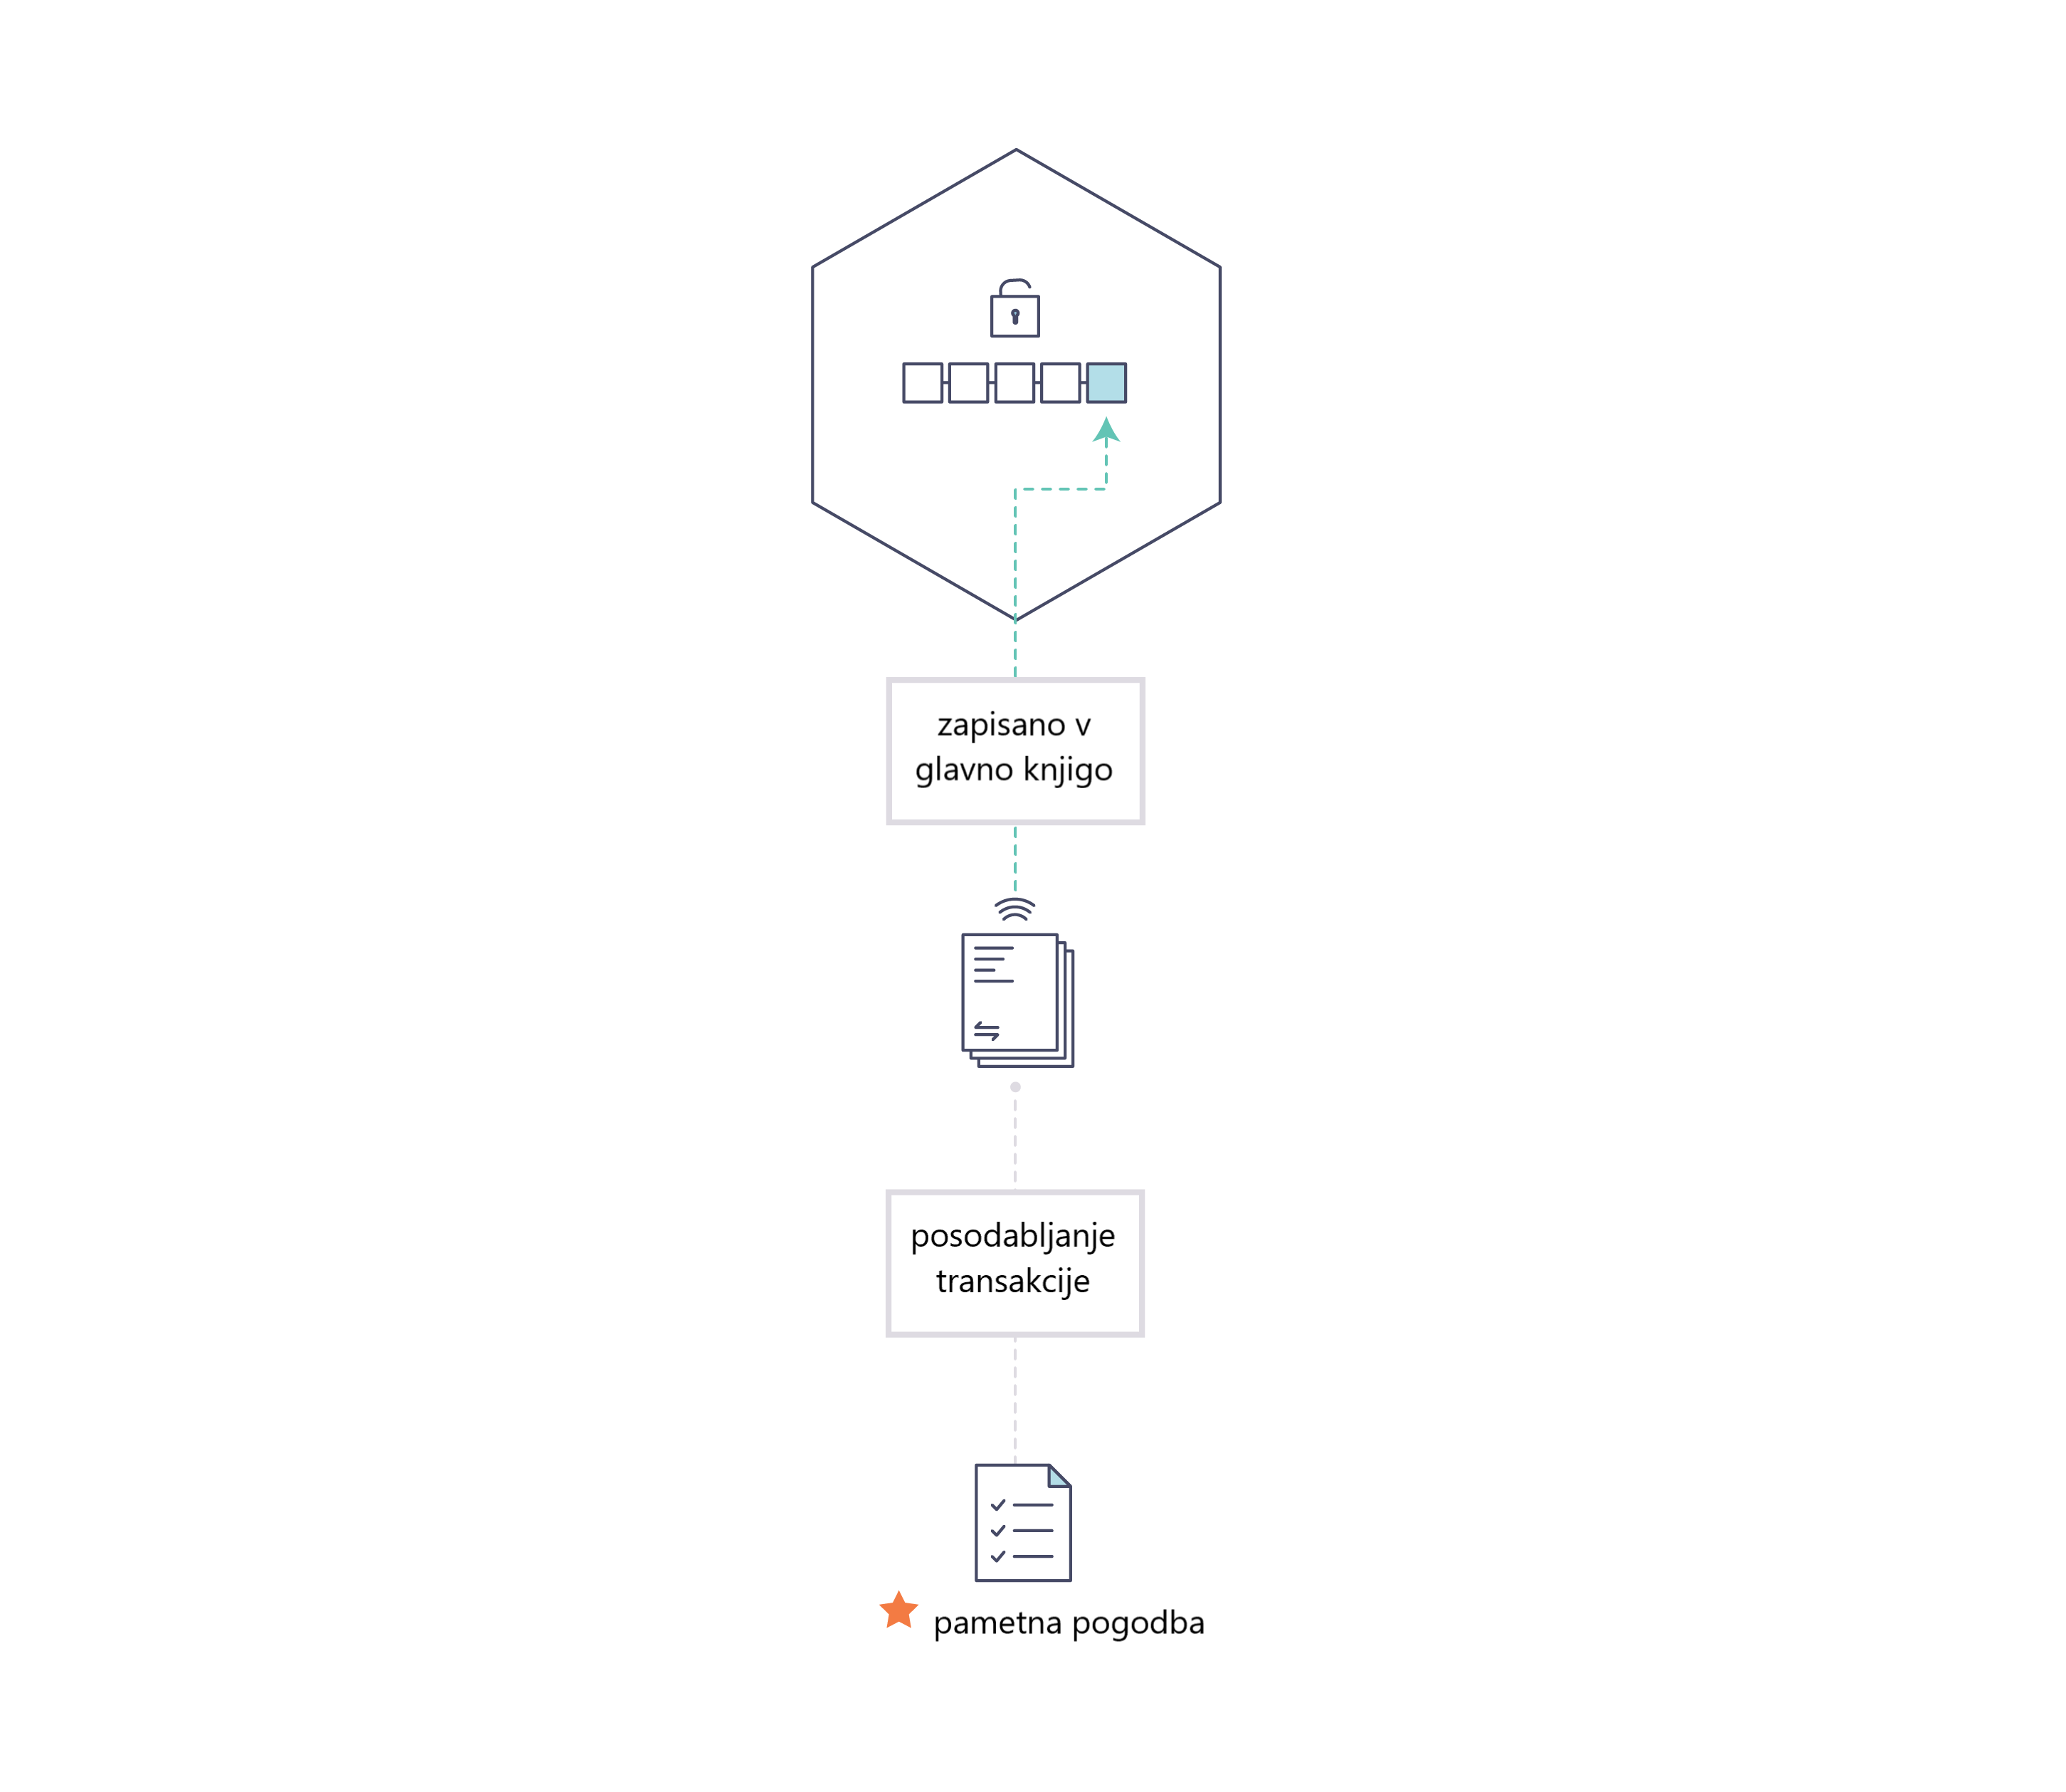
\includegraphics[width=1.0\textwidth]{slike/Smart_Contract_sl.png}
	\label{smart_contract}
	\caption{Interakcija pametne pogodbe z glavno knjigo \cite{hyperledgerDocs}.}
\end{figure}


\subsection{Soglasje}
Proces sinhronizacije glavne knjige v omrežju je imenovan soglasje.
Zagotavlja, da se glavna knjiga posodobi le takrat, ko so transakcije in podatkovni bloki potrjeni s strani zaupanja vrednih udeležencev omrežja.
Glavna knjiga se posodobi tako, da vsi udeleženci omrežja, izvedejo enake (zapisane) transakcije v istem vrstnem redu.
Slika \ref{consensus} grafično prikazuje primer doseženega soglasja.

\begin{figure}[h]
	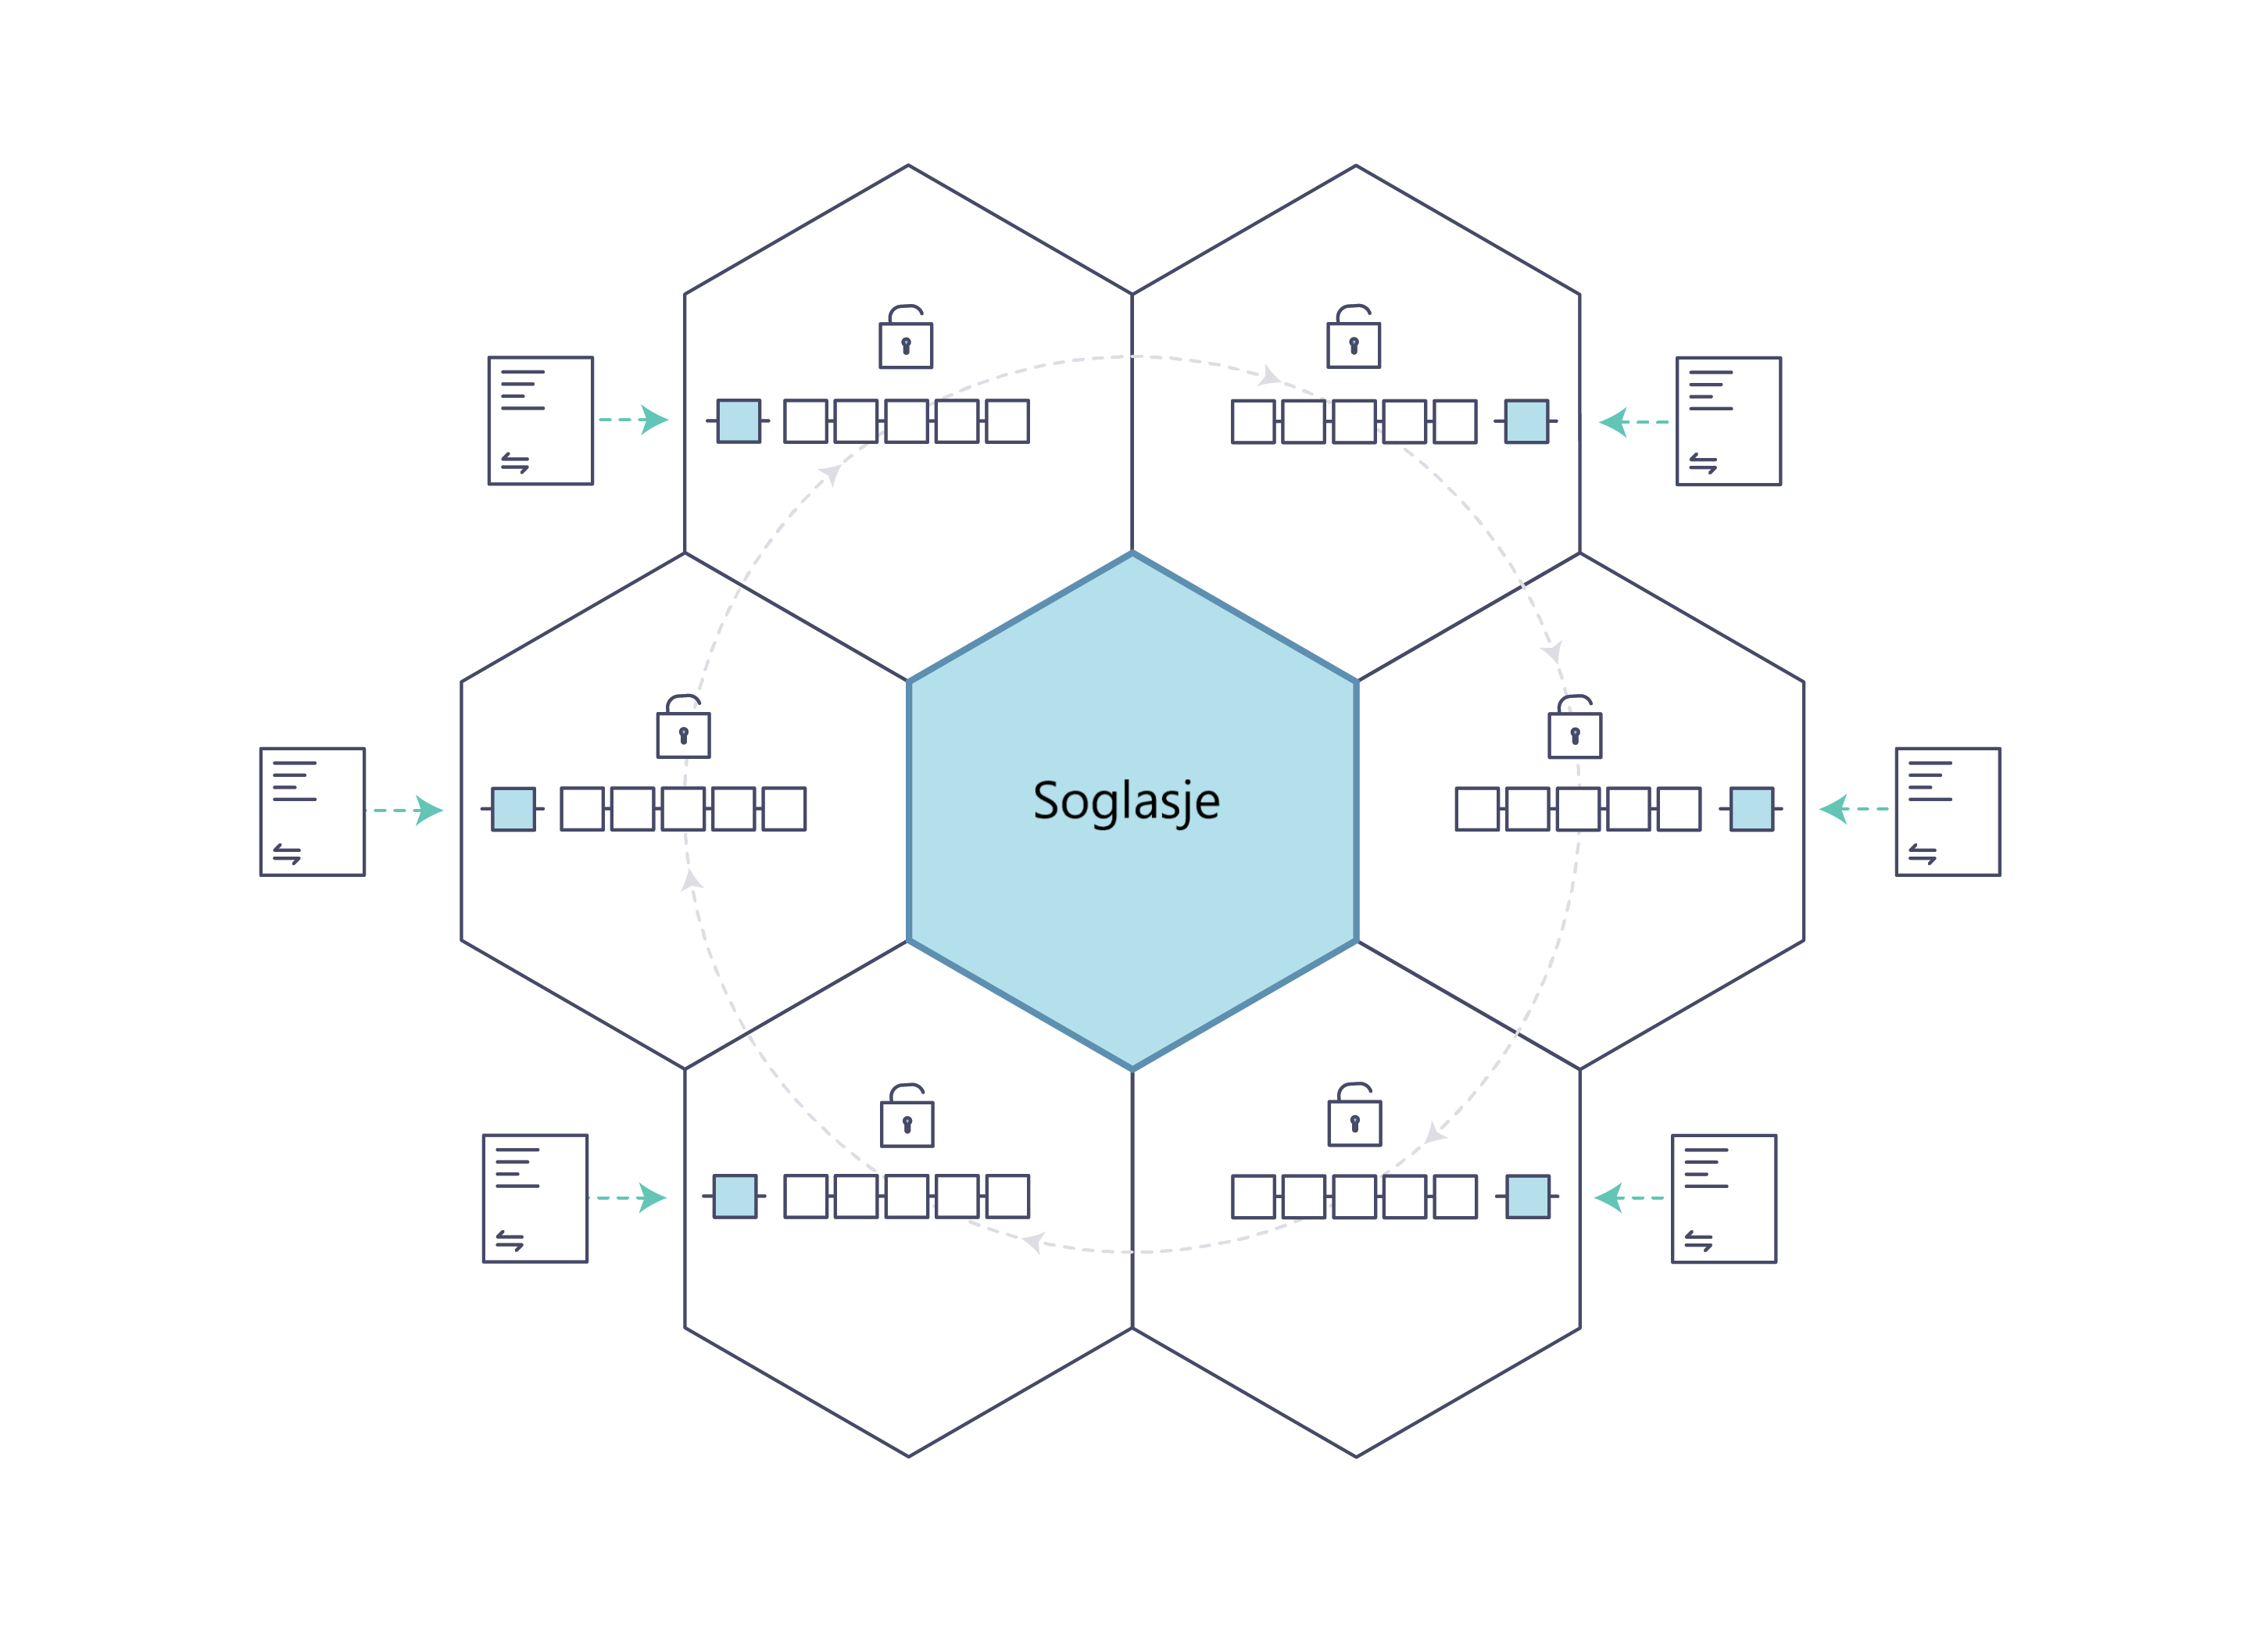
\includegraphics[width=1.0\textwidth]{slike/consensus.png}
	\label{consensus}
	\caption{Doseženo soglasje v omrežju \cite{hyperledgerDocs}.}
\end{figure}


\subsection{Izvajalna okolja glede na zaupanje med udeleženci}
V grobem lahko, glede na stopnjo zaupanja, ločimo dva tipa izvajalnih okolij, ki ga udeleženci delijo med seboj.
Imamo omrežje, kjer so udeleženci vnaprej znani, identificirani s strani tretje osebe, ki ji zaupajo vsi sodelujoči.
Interakcije med njimi so varne v smislu prevzemanja odgovornosti.
Morebitna škodoželjnost udeleženca je enostavno kaznovana zaradi fizično overjenih oseb (pravnih ali fizičnih).

V javnih okoljih teh ugodnosti ne uživamo.
V omrežju lahko sodeluje kdorkoli in to povsem anonimno,
med udeleženci tako privzeto velja načelo nezaupanja.
Zaupa se le stanju celotne podatkovne verige.
Tipično so za potrjevanje blokov in novih transakcij uporabljene \sn{kripto valute}, pridobljene s ti. postopkom rudarjenja.
Ta omrežja večinoma temeljijo na Byzantine Fault-Tolerance (BFT) \cite{hyperledgerDocs, castro1999practical}.

\subsection{Zasebnost in zaupnost}
Javne podatkovne verige so replicirane na vseh sodelujočih entitetah, kar prinaša transparentnost, obenem pa poslovnim subjektom onemogoča učinkovito sklepanje dodatnih ugodnosti, aneksov ipd. s poslovnimi partnerji.
Ena od možnih rešitev problema je enkripcija podatkov, ki pa v tem primeru odpove.
Vsak izmed sodelujočih ima dostop do celotne glavne knjige, kar omogoča enostavne napade s silo.
V nadaljanju predstavljeno omrežje Fabric tu vpeljuje koncept kanalov.
Ti predstavljajo logično grupiranje posameznih entitet in omejujejo dostop do pametnih pogodb in glavne knjige na posameznem kanalu \cite{hyperledgerDocs}.

\section{Ethereum}
Ethereum je decentralizirana platforma, ki izvaja pametne pogodbe (smart contracts) - aplikacije, ki se izvajajo natanko tako, kot so bile zapisane.
Platforma je osnovana na verigi podatkovnih blokov, ki omogoča reprezentacijo in prenos vrednosti.
Lahko si ga predstavljamo kot svetovni računalnik, izvajanje programske kode pa poteka na vseh sodelujočih računalnikih.
Pametne pogodbe ponujajo možnost interakcije s podatkovno verigo, določeni deli kode pa se izvajajo le pod točno določenimi pogoji \cite{ethereumWhitepaper}.

Stanje v Ethereum omrežju določajo objekti, znani kot uporabniški računi (accounts).
Vsak račun sestavlja 20 bajtov dolg naslov, prenos sredstev in informacij med računi pa predstavlja spremembo trenutnega stanja.
Uporabniške račune sestavljajo štiri polja \cite{ethereumWhitepaper}:
\begin{itemize}
\item števec (nonce), ki preprečuje podvajanje transakcij
\item trenutno stanje Ethra (ether balance) trenutna količina ethra v lasti računa
\item pogodbena koda (contract code) opcijska
\item shramba (storage) privzeto prazno
\end{itemize}

Ether je interno plačilno sredstvo v omrežju.
Uporablja se kot nadomestilo za izvrševanje transakcij.
Ethereum pozna dva tipa uporabniških entitet: zunanje (externally owned), določenih s privatnimi ključi in pogodbene (contract accounts), določenih s kodo.
Zunanji računi ne obvladujejo kode, z ostalimi entitetami v omrežju pa lahko komunicirajo preko digitalno podpisanih transakcij.
Pametne pogodbe so entitete, ki se v omrežju odzivajo na vnaprej določena sporočila: izvedejo del logike, berejo in pišejo v glavno knjigo oziroma pošljejo novo sporočilo v omrežje \cite{ethereumWhitepaper}.

\subsection{Komunikacija med entitetami}
V omrežju obstajata dva načina komunikacije: sporočila (messages) in transakcije (transactions).
Transakcije so podpisani podatkovni bloki, ki jih ustvarijo zunanji uporabniški računi.
Sestavni deli transakcije so:
\begin{itemize}
	\item prejemnik
	\item podpis pošiljatelja
	\item količina prenesenega ethra
	\item podatki (opcijsko)
	\item STARTGAS največje dovoljeno število izvedenih računskih operacij
	\item GASPRICE cena posamezne računske operacije
\end{itemize}

Sporočila so namenjena interni komunikaciji med pametnimi pogodbami.
So le navidezni objekti, obstajajo izključno v izvajalnem okolju.
Sestavlja jih \cite{ethereumWhitepaper}:
\begin{itemize}
	\item pošiljatelj
	\item prejemnik
	\item količina prenesenega ethra
	\item STARTGAS
\end{itemize}


\subsection{Navidezni stroj Ethereum}

Navidezni stroj je glavna abstrakcija celotnega omrežja.
Je izvajalno okolje za pametne pogodbe v Ethereum omrežju in služi kot \sn{peskovnik} za izvajanje kode.
Celotni navidezni stroj lahko predstavimo s terko \textbf{(stanje blokov, transakcija, sporočilo, koda, spomin, sklad, programski števec, plin)}.
\textit{Stanje blokov} je predstavitev vseh računov s trenutnim stanjem ethra in shrambe.
Vsaka izvedena operacija zmanjša vrednost preostale količine plina, glede na uteženost posamezne operacije.
Transakcija se zaključi ob izvedbi zadnje operacije v programu oziroma s prekinitvijo, ko porabljena količina plina preseše največjo dovoljeno \cite{ethereumWhitepaper}.


\subsubsection{Potrjevanje in kreiranje blokov}
Vsak blok v Ethereum verigi vsebuje kopijo vseh transakcij in zadnjega stanja omrežja.
Poleg tega sta v bloku zapisani tudi zaporedna številka bloka in zahtevnost.
Postopek validacije bloka poteka sledeče:
\begin{enumerate}
\item Preveri, če predhodni blok obstaja in je veljaven
\item Preveri časovni žig bloka - večji od prejšnejga bloka, vendar ne več kot 15 minut v prihodnosti
\item Preveri številko bloka, zahtevnost, izvor transakcije, izvor \sn{strica} in omejitev količine plina
\item Preveri veljavnost \sn{Proof of Work}
\item Naj bo S[0] stanje na koncu predhodnega bloka
\item Naj bo TX seznam transakcij v bloku. Za vsak 
$\{i \mid 0,1,\dots, n-1\}$
je naslednje stanje
 $S[i+1] = APPLY(S[i], TX[i])$.
V primeru napake ali presežene omejitve količine plina na blok (GASLIMIT), vrni napako.
\item Naj $S_FINAL = S[n]$. Nagrada za najden blok se izplača samo najditelju.
\item Preveri, da je vrhnje vozlišče Merklovega drevesa stanja $S_FINAL$ enaka končnemu stanju v bloku. V tem primeru je blok veljaven.
\end{enumerate}

Koda je izvedena s strani vseh sodelujočih entitet v omrežju \cite{ethereumWhitepaper}.

\section{Hyperledger}
Hyperledger je družina odprtokodnih projektov, namenjenih razvoju tehnologije veriženja podatkovnih blokov.
Projekt deluje pod okriljem organizacije The Linux Foundation, v sodelovanju s skupnostjo.
Med prvimi in najbolj znamimi izmed Hyperledger projektov je Hyperledger Fabric, prvotno razvit v podjetju IBM in Digital Asset.
Pod okrilje projekta Hyperledger spadajo še Sawtooth, Iroha, Burrow ter Indy.
Vsak izmed projektov na svoj način rešuje izzive s področja podatkovnih verig ali pa naslavlja ozko problemsko domeno. Kot primer: projekt Indy se ukvarja s problematiko spletne identitete uporabnika \cite{hyperledgerWeb}.
Trenutno najbolj znana in razširjena platforma je Fabric, trenutno v različici 1.1.
Od ostalih podobnih projektov se loči predvsem v konceptu privatnih omrežjih, pri katerih je sodelovanje omejeno s sistemom dovoljenj.
Omogoča modularno izbiro načina soglasja in ga je moč prilagajati zahtevam poslovnih uporabnikov \cite{hyperledgerIbm}.

\subsection{Fabric}
Hyperledger Fabric je v sami zasnovi namenjen poslovni uporabi.
Omogoča modularno in prilagodljivo arhitekturo, podobno kot ostale implementacije tehnologije veriženja blokov pozna tudi pametne pogodbe, tu imenovane \sn{chain code}.
Pametne pogodbe se tu izvajajo znotraj vsebnikov Docker in omogočajo implementacijo v poljubnem splošnonamenskem programskem jeziku.
Drugačen je tudi postopek izvedbe transakcije.

Celotno omrežje je zasnovano na predpostavki (delnega) zaupanja med sodelujočimi entitetami, za razliko od javnih omrežij.
Enostavna je menjava implementacije protokola za doseganje soglasja, bodisi na osnovi reševanja napak ob odpovedi (Crash Fault Tolerant -- CFT) ali bizantinske odpornosti na napake (Byzantine Fault Tolerance -- BFT).
Za samo delovanje ne potrebuje kriptovalute, potrjevanje transakcij in blokov pa ni nujno izvedeno s strani vseh sodelujočih, ampak le določene podmnožice, kar v teoriji omogoča paralelizacijo in posledično višjo zmogljivost \cite{hyperledgerDocs}.

\subsubsection{Modularnost}
Omrežje sestoji iz šestih osnovnih komponent, ki jih je moč poljubno menjati \cite{hyperledgerDocs}:
\begin{enumerate}
	\item urejevalnik (ordering service)
	\item upravitelj članstva (membership service) - povezuje zunanje entitete z njihovimi kriptografskimi predstavitvami
	\item P2P gossip protocol - opcijski
	\item Pametne pogodbe (chaincode) - procesno izolacijo zagotavlja izvajanje znotraj vsebnikov Docker. 
	Onemogočen je neposreden dostop do glavne knjige
	\item SUPB (DBMS)
	\item zamenljiva politika potrjevanja in validiranja
\end{enumerate}

\subsubsection{Pametne pogodbe}
Pametne pogodbe so delčki programske kode, ki se izvajajo kot distribuirane aplikacije.
Tri glavne značilnosti teh aplikacij so: veliko število sočasno izvajanih pametnih pogodb, dinamično dodajanje v omrežje in v osnovi nevredne zaupanja.
Obstoječi načini izvajanja pogodb so umeščene v arhitekturo \textbf{uredi-izvedi}.
Za njih je značilno, da transakcije validirajo in sekvečno uredijo, temu pa sledi propagacija potrjenih blokov po omrežju.
Vsaka sodelujoča entitea nato transakcije izvede v tem vrstem redu.
Za enoličen način sekvenčnega izvajanja tu nastane potreba po novem, determinističnem programskem jeziku.
En izmed predstavnikov je programski jezik za programiranje pogodb v omrežju Ethereum, Solidity.
Ker je vsaka izmed transakcij izvedena s strani vsake entitete, to predstavlja veliko porabo razpoložljivih virov ter omejuje skaliranje ter učinkovitost izvajanja \cite{hyperledgerDocs}.

Fabric pametne pogodbe izvaja po arhitekturi \textbf{izvedi-uredi-validiraj}.
Vsaka transakcija je najprej izvedena s čimer se preveri njeno pravilnost.
Nato je urejena, glede na protokol za doseganje soglasja.
Ob koncu je transakcija validirana s strani za to pooblaščenih zunanjih entitet.
Tu v igro vstopi domensko specifična politika potrjevanja.
Slednje prinaša potencialno velike performančne prihranke \cite{hyperledgerDocs}.

\section{Tehnologija veriženja podatkovnih blokov v kontekstu decentraliziranega izvajanja}
Decentralizirana hramba podatkov je osnova, na kateri je primerno graditi in osnovati sisteme, sposobne decentraliziranega izvajanja.
Raziskave in tehnike uporabe kriptografskih in drugih protokolov, ki zagotavljajo nespremenljivost podatkov in v praksi tudi njihovo ponarejanje, lahko apliciramo nivo višje, v poslovno logiko.
Trenutno znamo varno hraniti podatke na tisoče napravah, ter hkrati zagotavljati njihovo pristnost.
Svoje zamisli o decentraliziranem registru sem osnoval prav na tej pomembni pridobitvi, kar bom podrobneje razložil v poglavju \ref{ch4}.

\chapter{Decentralizirano izvajanje}
\label{ch4}

Izvajanje storitev se danes seli v oblak.
Ta način izvajanja s seboj prinaša kar nekaj prednosti, kot so samodejno skaliranje in istanciranje posamezne storitve, glede na trenutne zahteve in potrebe.
Računalniški oblak je abstrackija, ki za seboj skriva ogromne podatkovne in računske centre.
Ti so v večini v lasti velikih korporacij, prednjačijo Amazon, Google in Microsoft.
Odvisnost od ponudnika računalniškega oblaka zna biti problematična, napaka v sistemu lahko povzroči večurno nedostopnost naših storitev. 
Navkljub skrbi, ki jo ponudniki posvečajo vzdrževanju 100\% dosegljivosti, od zadnjega odmevnejšega primera mineva le dobro leto in pol \cite{awsFail}.

Izvajanje storitev želimo decentralizirati - vsaka sodelujoča entiteta v omrežju lahko, pod določenimi pogoji, izvaja katerokoli izmed nabora razpoložljivih storitev.
Prednost, ki jo prinaša decentralizirano izvajanje poslovne logike je praktično nemogoč napad zavrnitev storitve (DOS) in porazdeljen napad zavrnitve storitve (DDOS).
Napadalec je zmožen posamezno sodelujočo entiteto v omrežju obremeniti do te mere, da le ta preneha z izvajanjem določene storitve.
Decentraliziran sistem bi v primeru prenehanja izvajanja storitve na eni entiteti izvajanje dodelil drugi. Postopek bi moral biti za končnega uporabnika storitve transparenten.
S tehnologijo podatkovnih blokov bi bilo moč posamezne klice storitev tudi finančno ovrednotiti.
Trenutno je potrebnih več klicev, ki kot prvo izvedejo samo poslovno logiko aplikacije, temu pa sledi klic, ki izvede še finančno transakcijo.
Podatkovna veriga nam omogoča, da klice storitev opremimo s finančnimi podatki in ob uspešni izvedbi izvajalca sistem samodejno nagradi.

V nadaljevanju diplomskega dela so predstavljeni osnovni koncepti rešitve registracije in odkrivanja storitev v decentraliziranem okolju.
Odkrivanje storitev v decentraliziranem okolju igra prav tako pomembno vlogo, kot pri storitvah, ki se izvajajo v oblačnih sistemih.
Predstavljena rešitev predstavlja le del celotnega sistema, ki bo omogočal decentralizirano izvajanje.

\section{Odkrivanje storitev v decentraliziranem okolju}
Predlagana zasnova sistema za odkrivanje storitev v decentraliziranem okolju sestoji iz naslednjih komponent:
\begin{itemize}
	\item Registracija nove aplikacije \ref{registerService}
	\item Registracija izvajalcev \ref{registerWorker}
	\item Registracija storitve \ref{registerExecution}
	\item Odkrivanje storitev \ref{serviceDiscovery}
\end{itemize}

Registracija in odkrivanje storitve je uporaba že znanih konceptov, prenesenih v okolje, kjer vlogo registra storitev prevzema porazdeljena glavna knjiga.
Dodatno smo uvedli še registracijo aplikacije, ki je pripravljena na izvajanje v decentraliziranem omrežju in registracijo izvajalcev.
Slednja omogoča lastništvo več izvajalnih naprav eni posamezni identiteti.


\subsection{Registracija nove aplikacije}
\label{registerService}

Omrežje je javno, kdorkoli lahko objavi in ponudi novo aplikacijo, pripravljeno za izvajanje.
Izvorno kodo oziroma izvršljivo datoteko aplikacije shranimo v decentralizirano shrambo.
Temu sledi zapis podatkov (ime, verzija, izvajalno okolje...) o aplikaciji v glavno knjigo.
Ob uspešni registraciji omrežje proži dogodek s podatki o novi aplikaciji.
Posamezni izvajalec, ki se registrira na te dogodke, lahko takoj prične z izvajanjem aplikacije, če se za to odloči, oziroma mu izvajanje dodeli omrežje.
Razporejanje opravil in izvajanja po omrežju je stvar prihodnjih raziskav.
Preprost diagram poteka je prikazan na sliki \ref{register_api}.

\begin{figure}[h]
	\centering
	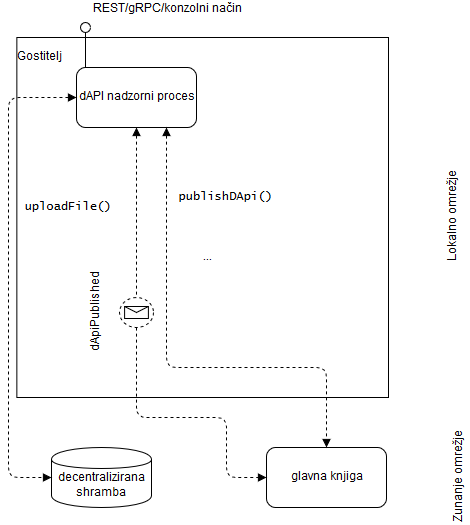
\includegraphics[width=0.8\textwidth]{slike/register_api.png}
	\label{register_api}
	\caption{Registracija nove aplikacije}
\end{figure}

\subsection{Registracija izvajalcev}
\label{registerWorker}
Vsaka identiteta lahko upravlja z več izvajalnimi enotami.
Ta pristop omogoča enemu uporabniškemu računu pripis vseh nagrad, ki si jih posamezni izvajalec prisluži.
Podatki, ki se o posameznem izvajalcu zabeležijo so: lastnik (account), unikatna številka izvajalca (id) in naslov, preko katerega je izvajalec dosegljiv.
Izvajalcu se lokalno konfigurira omejitve glede porabe sistemskih virov, ki jih lastnik nameni decentraliziranemu izvajanju storitev.
Postopek je shematsko prikazan na sliki \ref{register_worker}.

\begin{figure}[h]
	\centering
	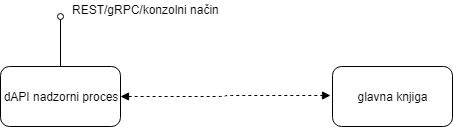
\includegraphics[width=1.0\textwidth]{slike/register_worker.png}
	\label{register_worker}
	\caption{Postopek registracije izvajalcev}
\end{figure}

\subsection{Registracija izvajanja storitve}
\label{registerExecution}
Ob zahtevi za pričetek izvajanja aplikacije, ki je bila predhodno registrirana v omrežju, se prične postopek pridobivanja informacij o želeni storitvi.
Iz registra aplikacije se pridobi podatke o imenu, verziji, lastniku in lokaciji shrambe.
Izvorno kodo oz. izvršljivo datoteko storitve se nato pridobi iz omrežja, po potrebi jo nadzorni proces prevede in zažene.
Storitev sama ob inicializaciji poskrbi za registracijo v registru (glavna knjiga).
Zabeleži se podatke o izvajalcu in storitvi, ki je pričela z izvajanjem.
Gre za najbolj kompleksen del registracije, shematsko je prikazan na sliki \ref{register_service}.

\begin{figure}[h]
	\centering
	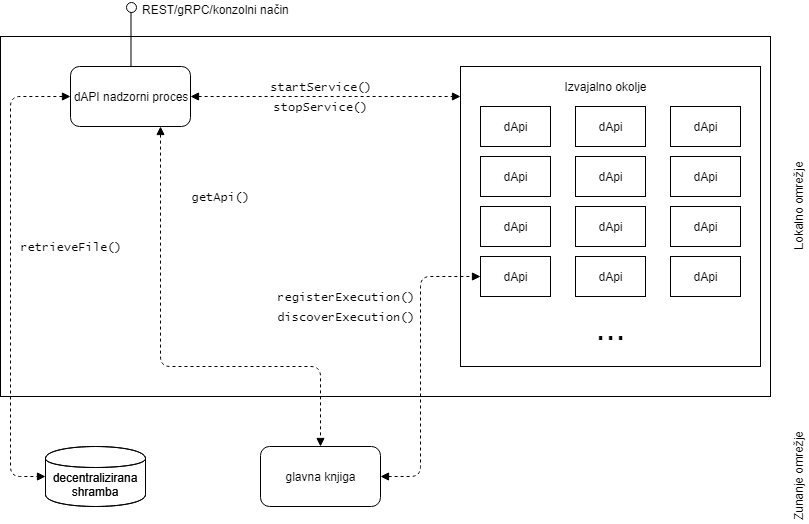
\includegraphics[width=0.8\textwidth]{slike/register_service.png}
	\label{register_service}
	\caption{Postopek registracije izvajanja storitve}
\end{figure}

\subsection{Odkrivanje storitve}
\label{serviceDiscovery}
Želeno storitev, pod pogojem, da se v omrežju izvaja, pridobimo z enostavno poizvedbo v glavni knjigi.
Med razpoložljivimi storitvami odjemalec izbere eno, pridobi podatke o lokaciji izvajanja in izvede klic \ref{discover_service}.
Od tu naprej komunikacija med storitvami poteka preko izbranega protokola (REST, gRPC, Event-driven).

\begin{figure}[h]
	\centering
	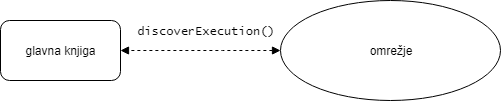
\includegraphics[width=0.8\textwidth]{slike/discover_service.png}
	\label{discover_service}
	\caption{Postopek odkrivanja}
\end{figure}

Deregistracija storitev predstavlja težji del naloge, ker ni centralnega procesa, ki bi bdel nad registriranimi storitvami in preverjal njihovo dosegljivost.
Potrebna bo dodatno raziskovalno delo, kako učinkovito deregistrirati storitev, podobno kot je to rešeno pri trenutno uporabljenih registrih (etcd, Consul, ZooKeeper).
Za deregistracijo posamezne storitve je tako zaenkrat odgovoren nadzorni proces.

\chapter{Implementacija predlagane rešitve}
\label{ch5}

Pri implementaciji predstavljenih konceptov sem se osredotočil le na osnovne funkcionalnosti registra - registracijo aplikacije, registracijo izvajalcev in registracijo storitve.

\begin{figure}[h]
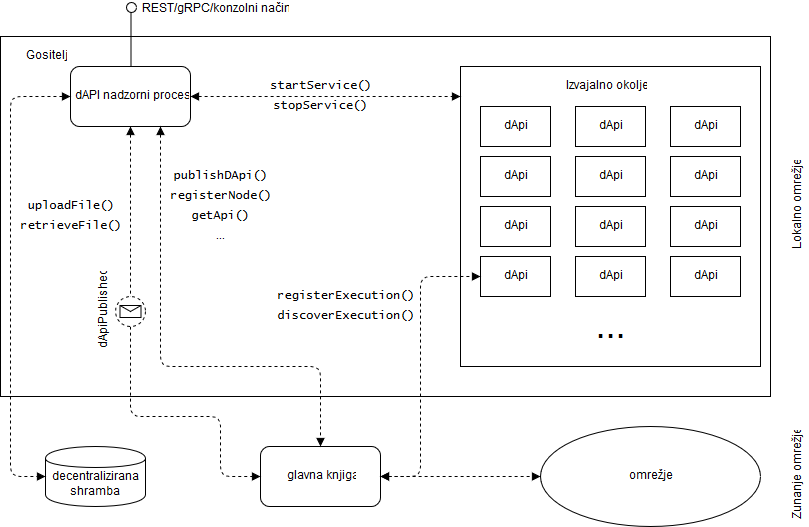
\includegraphics[width=0.8\textwidth]{slike/dApi_sl.png}
\label{scheme}
\caption{Arhitekturna shema rešitve}
\end{figure}

Na sliki \ref{scheme} je prikazana shema predlagane rešitve. Osrednji del omrežja je nadzorni proces - 
dApi manager, ki dostopa do glavne knjige, decentralizirane shrambe in upravlja s storitvami, ki jih gostitelj izvaja.
Gostiteljski sistem v trenutni različici podpira upravljanje z vsebniki Docker.
Aplikacije, ki so na voljo za izvajanje so shranjene na datotečni shrambi IPFS, podporna podatkovna veriga je na omrežju Ethereum. Posamezne komponente sistema so podrobneje opisane v nadaljevanju.

\section{Nadzorni proces}
Nadzorni proces za izvajanje decentraliziranih storitev (dAPIjev) skrbi za:
\begin{itemize}
	\item registracijo novih storitev v omrežje, 
	\item prenos izvršljivih datotek v in iz omrežja,
	\item zagon, zaustavitev in upravljanje storitev
\end{itemize}

Komunikacija z nadzornim procesom trenutno poteka preko REST aplikacijskega vmesnika, v načrtu pa je implementacija vmesnikov za konzolni nadzor ter podpora novejšim komunikacijsim protokolom kot so gRPC, Apache Trift in podobni.

Za registracijo nove storitve nadzornemu procesu podamo pot do slike vsebnika Docker.
Sistem poskrbi za distribucijo slike v omrežje IPFS in podatke o storitvi doda v shrambo pogodbe na Ethereum omrežju.
Ob uspešni registraciji se proži dogodek, ki sodelujoče entitete obvesti o novi storitvi, pripravljeni na izvajanje.
Te se lahko na dogodek lahko odzovejo z zahtevo za izvajanje storitve.
Trenutno je izvajanje nove storitve potrebno prožiti ročno, ko bo pripravljen modul za razporejanje opravil, bo postopek v celoti avtomatiziran.
Pred pričetkom izvajanje se želeno storitev pridobi iz omrežja (IPFS), sliko vsebnika naloži v izvajalno okolje Docker in proži izvajanje.
Storitev nato sama poskrbi za registracijo in odkrivanje ostalih storitev v omrežju.

Razširitev obstoječe KumuluzEE konfiguracijske datoteke:

\begin{lstlisting}
dapi-manager:
  storage:
    remote:
      type: ipfs
      location: /ip4/127.0.0.1/tcp/5001
    local:
      downloadFolder: download
      execution:
  managers:
  - type: docker
    connection: tcp://192.168.99.100:2376
    tls: true
    certificate-path: /path/to/certificate
    instance-limit: 10
  blockchain:
    provider: ethereum
    host: http://127.0.0.1:8545
    account: /path/to/wallet
    password: password
\end{lstlisting}

\section{Decentralizirana shramba}
Izvršljive datoteke oziroma slike vsebnikov storitve je potrebno shraniti na način in lokacijo, kjer bodo dostopne vsem sodelujočim entitetam v omrežju.
Podobno, kot želimo izvajanje storitev decentralizirati, moramo poskrbeti tudi za decentralizirano shrambo.
V svoji implementaciji sem uporabil decentralizirano shrambo IPFS.
Gre za projekt, osnovan na omrežju Ethereum, namen projekta pa je shranjevanje datotek v porazdeljeni shrambi, dostop do njih pa preko omrežji P2P, podobno kot deluje protokol BitTorrent, po katerem se projekt tudi zgleduje.
Vsako datoteko, ki jo želimo shraniti v omrežje, odjemalec razbije na podatkovne bloke, izračuna zgoščeno vrednost posameznega bloka, te vrednosti pa nato sestavi v strukturo imenovano Merkle Tree.
Datoteko pridobimo enostavno preko zgoščene vrednosti v korenu drevesa.
Omrežje je sposobno poiskati posamezne koščke prvotne datoteke, vsebino posameznega pa hitro preveri z izračunom zgoščene vrednosti. V kolikor nam kdo želi podtakniti napačne bloke posamezne datoteke, sistem to prepozna in neveljavne bloke preprosto zavrže, ko od ostalih sodelujočih entitet prejme iste dele datoteke. Datoteka je veljavna, v kolikor sistem uspe sestaviti podatkovno strukturo Merkle Tree, katerega zgoščena vrednost v korenu drevesa je identična podani \cite{Ipfs}.

\section{Odjemalec za Ethereum omrežje}
Sistem za delovanje potrebuje odjemalca, ki se zna povezati v Ethereum omrežje.
V moji testni postavitvi je mesto odjemalca prevzel program Geth, implementacija Ethereum protokola v programskem jeziku Go. \cite{Geth}
Nadzorni proces se preko JSON RPC povezuje na lokalno instanco odjemalca Geth, decentralizirane storitve v izvajalnem okolju Docker pa se 
povezujejo na proces, dostopen preko mreže Infura.
Infura nam omogoča enostaven dostop do Ethereum omrežja, brez potrebe po lokalnem izvajanju Ehtereum protokola.
Za sodelovanje v Ethereum omrežju nam tako lokalno ni potrebno namestiti ničesar, prav tako nam ni potrebno hraniti
celotne zgodovine podatkovne verige. 
Na spletni strani se enostavno registriramo, s tem pridobimo unikaten ključ, ki nam omogoča dostop do oddaljenega izvajalca \cite{Infura}.

\section{Implementacija pametne pogodbe}
Pametna pogodba, ki predstavlja register storitev in osrednji del sistema, je napisana v programskem jeziku Solidity.
Solidity je jezik, v katerem ustvarjalci Ethereum omrežja priporočajo implementacije pametnih pogodb.
Je visoko nivojski jezik, precej podoben JavaScriptu in namenjen izvajanju na navideznem stroju Ethereum (EVM).
Med konstrukti jezika najdemo dedovanje, knjižnice, uporabniško določene tipe in ostale visokonivojske konstrukte.
Namensko orodje za razvoj pametnih pogodb je trenutno le eno, poznano pod imenom Remix, dostopno pa je tudi v spletni različici
\cite{solidityDocs}.

Osnovni konstrukti zasnovane pogodbe so strukture User, dApi, Worker in Execution.

\begin{lstlisting}
contract Registry {
	struct User {
		string friendlyName;
		mapping(bytes32 => Worker) workers;
		mapping(bytes32 => dApi) dApis;
	}
	
	struct dApi {
		string name;
		string version;
		string location;
		bool isValid;
	}
	
	struct Worker {
		string name;
		bytes32 workerId;
		bool isValid;
	}
	
	struct Execution {
		Worker worker;
		string location;
		bool active;
	}
	
 	/// MAPPINGS
	mapping (address => User) users;
	mapping (bytes32 => Execution[]) dAPIExecutors;
	...
\end{lstlisting}

Struktura \textbf{User} predstavlja ponudnika decentraliziranih aplikacij.
Vsakemu ponudniku pripada seznam izvajalcev (workers) in objavljenih APIjev (dApis).
O posamezni storitvi hranimo ime, verzijo ter lokacijo, ki v našem primeru predstavlja zgoščeno vrednost korena slike Docker, shranjene na IPFS.
Vsak izvajalec je samostjona enota, ki je zadolžena za izvajanje aplikacije, struktura Execution, v navezavi z mapiranjem \textit{dAPIExecutors} pa povezuje aplikacijo z njenimi izvajalci in naslovu, preko katerega je dostopna.

Registracija poteka v več korakih, najprej je potrebno registrirati ponudnika storitve, nato se samodejno, ob zagonu instance nadzorne storitve, izvede registracija izvajalca.
Za registracijo storitve poskrbi storitev sama, preko razširitve \textit{Kumuluz-dapi}, takoj ob zagonu.

\begin{lstlisting}
function registerApi(string _name,
	string _version,
	string _location,
	bytes32 _hash, bool _isValid) public {
	dApi memory dapi = dApi(
	_name,
	_version,
	_location,
	_isValid
	);
	
	users[msg.sender].dApis[_hash] = dapi;
	emit dAPIPublished(_name, _version, msg.sender,
	_hash);
}
...
\end{lstlisting}

Proces deregistracije izvajanja storitve je kompleksnejši postopek, ki zahteva kar nekaj računskega dela.
Dokler je v sistemu malo registriranih izvajalnih enot je deregistracija dokaj neopazna, tako z vidika časa in cene.
Problem nastopi v primeru velikega števila izvajalnih enot.
Na testnem omrežju \textit{Rinkeby} sem ob testiranju večjega števila registrianih izvajalnih enot presegel omejitev računskih korakov na transakcijo (gas).

\begin{lstlisting}
function deregisterExecution(bytes32 _apiHash, 
uint _wIndex) public {
	if (_wIndex >= dAPIExecutors[_apiHash].length)
		return;
	
	for (uint i = _wIndex;
	i<dAPIExecutors[_apiHash].length-1; i++){
		dAPIExecutors[_apiHash][i]=
			dAPIExecutors[_apiHash][i+1];
	}
	dAPIExecutors[_apiHash].length--;
}
\end{lstlisting}

Večji problem nastopi ob deregistraciji izvajalca, tu bi bilo potrebno iterirati preko vseh registriranih storitev in poiskati izvajalca za brisanje.
Ta del registra še ni implementiran in potrebuje dodatno pozornost v prihodnje.


\section{Razširitev KumuluzEE platforme za podporo decentraliziranim aplikacijam}

\subsection{Implementacija Kumuluz-dapi}
Želja in cilj za učinkovit razvoj decentraliziranih aplikacij je priprava programskih vmesnikov, ki bodo razvijalcem omogočili enostavno nadgradnjo in predelavo obstoječih aplikacij v dApije.
V razvojni fazi je razširitev za aplikacije, ki uporabljajo platformo KumuluzEE.
Vmesnik mora biti intuitiven in enostaven za uporabo, zato smo za zgled vzeli podobno in že obstoječo rešitev \textit{KumuluzEE Service Discovery}, ki rešuje problem odkrivanja storitev v oblačnih arhitekturah \cite{maldip}.

\subsubsection{Anotacije}
Razširitev vsebuje dve anotaciji, s katerima opremimo obstoječo aplikacijo.
Prva služi registraciji storitve, z njo pa se opremi glavni aplikacijski razred REST storitve, ki je trenutno edini podprt način komunikacije.

\begin{lstlisting}
@Qualifier
@Retention(RetentionPolicy.RUNTIME)
@Target({ElementType.TYPE})
public @interface RegisterDApi {
	String name() default "";
	String environment() default "";
	String version() default "";
	ApiType apiType() default ApiType.REST;
}
\end{lstlisting}

Podatki, ki jih beležimo o posamezni storitvi so: \textit{ime (name), okolje (environment), verzija (version) in tip aplikacijskega vmesnika (apiType)}.


Druga anotacija skrbi za označevanje parametrov, ki jih preko javanske tehnologije CDI, vrinemo v spremenljivke.

\begin{lstlisting}
@Qualifier
@Target({ElementType.FIELD, ElementType.METHOD})
@Retention(RetentionPolicy.RUNTIME)
public @interface DiscoverDApi {
	@Nonbinding String name() default "";
	
	@Nonbinding String environment() default "";
	
	@Nonbinding String version() default "";
	
	@Nonbinding ApiType apiType()
	 default ApiType.REST;
}
\end{lstlisting}

\subsubsection{Programska logika}
Preko procesiranja anotacij pridobimo podatke o želeni storitvi, pri inicializaciji pa razširitev poskrbi za samodejno registracijo, oziroma odkrivanje storitve.
Za delovanje razširitve potrebujemo omogočeno tehnologijo CDI.
Metoda za registracijo storitve je povsem enostavna, uporabljamo pa knjižnico Web3j.
Web3j je majhna knjižnica, namenjena aplikacijam Java in Android, ki se zna povezati na omrežje Ethereum.
Klice na REST vmesnik odjemalca (geth, parity) ovije v razrede in metode, omogoča pa tudi pretvorbo pogodb v jeziku Solidity v javanske razrede \cite{web3j}.

\begin{lstlisting}
private void registerService(
	ServiceExecution apiExecutionDetails) {
	
	logger.info("Registering new service execution");
	registry
	.registerService(apiExecutionDetails.getApiHash(),
	 apiExecutionDetails.getWorker(),
	 apiExecutionDetails.getLocation()).observable()
	.subscribe(tx -> {
	BigInteger gasUsed = tx.getGasUsed();
	logger.info("New dApi executor registered: "
	 + apiExecutionDetails.toString() + 
	 ". Gas spent: " + gasUsed);
	logger.info("Block number: "
	 + tx.getBlockNumber());
	});
}
\end{lstlisting}



\subsection{Priprava aplikacije}
V standardno KumuluzEE aplikacijo je potrebno vključiti razširitev \textit{kumuluz-dapi}. 
Razširitev ponuja nabor anotacij, s katerimi storitev bodisi registriramo v omrežje, bodisi določeno storitev poiščemo.
Potrebna je še dopolnitev konfiguracijske datoteke, v kateri podamo dodatne informacije o naši storitvi.
Ob zagonu storitve se preko anotacij poišče in registrira v omrežje.
V glavno knjigo se zapišejo podatki o izvajani storitvi, izvajalcu ter naslov, na katerem je storitev dostopna.

Za odkrivanje storitev poskrbi razširitev, ki v glavni knjigi poišče izvajalce storitve, med njimi pa na podlagi izbranega algoritma za razporejanje bremena, izbere enega izmed izvajalcev in pridobi naslov, na katerem se storitev trenutno izvaja.

Razširitev obstoječe KumuluzEE konfiguracijske datoteke:
\begin{lstlisting}
  dapi:
    blockchain:
      host: naslov izvajalca
      account: /pot/do/datoteke
      password: geslo
    type: docker
    storage: ipfs
    api: rest
\end{lstlisting}

V konfiguraciji so predvidene tudi trenutno neuporabljene nastavitve za tip izvršljive datoteke, v kateri shrambi se storitev nahaja in tip aplikacijskega vmesnika.
Trenutno sistem podpira le vsebnike Docker, ki jih je moč pridobiti preko omrežja IPFS, aplikacijski vmesnik pa je REST.


\chapter{Delovanje in evalvacija}

\section{Testna aplikacija}

Za namene testiranja delovanja sistema sem implementiral dve preprosti REST storitvi - uporabniki (users) in kupci (customers).
Storitev \textit{uporabniki} hrani seznam vseh uporabnikov v sistemu.
Storitev \textit{kupci} od prve storitve pridobi seznam uporabnikov in ga le posreduje naprej.
Prva storitev testira uspešnost registracije izvajanja, medtem ko druga služi kot test odkrivanja uspešno registrirane storitve.

Implementirani storitvi sta zelo enostavni, sestavljata ju le po dva Javanska razreda, zato jih na tem mestu ne bi posebej predstavljal.

\section{Testiranje}
Celotnega sistema nisem uspel spraviti v popolnoma delujoče stanje, zaradi težav in pomankljivosti, ki so podrobno navedene v podpoglavju \ref{improvments}.
Ob zagonu nadzornega procesa se uspešno le-ta uspešno registrira kot izvajalec.
Zatem s klicem na \textit{/dapi/{account}/registerApi} uspešno prenese sliko Docker na shrambo IPFS in programski vmesnik registrira na omrežje.
Uspešno se izvede tudi proženje dogodka, ki sodelujoče obvesti o novo objavljeni storitvi.

S klicem na \textit{/dapi/{address}/startService} se iz shrambe IPFS prenese slika aplikacije, vendar je le ta poškodovana in je ni moč naložiti ter izvesti.
Sistem sem ročno zaobšel in preko nadzornega procesa zagnal lokalno kopije slike.
Storitev se uspešno zažene in registira v omrežju, tu pa nastopi naslednja težava.
Storitev je moč odkriti, vendar ne takoj po registraciji.
Vzroka za to nisem uspel najti, ko pa je storitev moč odkriti, se testna aplikacija \textit{kupci} uspešno poveže na storitev \textit{uporabniki} in ob zahtevi pridobi celoten seznam uporabnikov, ki ga le posreduje naprej.


\section{Pomankljivosti trenutnega sistema in izboljšave v prihodnosti}
\label{improvments}

Prva različica sistema ponuja kar nekaj možnosti za izboljšave.
Prva izmed pomankljivosti je sama cena registracije in deregistracije storitev in njihovih izvajalcev.
Vsaka registracija novega izvajalca pomeni nov zapis na podatkovno verigo, kar v dinamičnem sistemu in ob trenutnih cenah transakcije na Ethereum omrežju predstavlja potencialno veliko finančno breme za izvajalca.
Zahtevnejša od prve je druga pomankljivost sistema in sicer deregistracija izvajalca.
Brisanje podatkov iz podatkovne verige je nemogoče zaradi same zasnove tehnologije - nespremenljivost.
S transakcijo je možno le navidezno brisati - razveljaviti preteklo transakcijo, zapis pa na podatkovni verigi ostane.
Brisanje je prav tako razmeroma draga operacija, posebno velik problem predstavlja brisanje izvajalca in s tem posledično še deregistracijo vseh storitev, ki jih je ta izvajalec v trenutku prekinitve izvajanja izvajal.

Dodatni mehanizmi, ki jih poznajo obstoječi sistemi za odkrivanje storitev, so še samodejna deregistracija storitve ob vnaprej določenem pretečenem času neaktivnosti.
Trenutna implementacija tega mehanizma še ne pozna, problem predstavlja predvsem decentralizacija.
V tem sistemu ne poznamo centralne storitve, ki bi ob določenem času iz registra preprosto brisala vse neaktivne storitve.
Sistem potrebuje nov mehanizem, ki bo znal med storitvami poiskati neaktivne in jih odstraniti iz registra. Kakšen bo mehanizem in princip delovanja sta v tem trenutku neznanka.

Sistem potrebuje tudi način prerazporejanja zahtev po omrežju.
Kdo izmed trenutno registriranih izvajalcev bo lahko najhitreje odgovoril?
Hiter odgovor je pogojen s fizično oddaljenostjo gostitelja od izvajalca, omrežnimi zakasnitvami, hitrost samega izvajalca. Reševanje teh izzivov je naslednja v vrsti, ki jih predstavlja celostna postavitev, v praksi uporabnega, sistema.


Vsakega izvajalca storitve želimo za uspešno izveden klic ustrezno finančno nagraditi. Tu se poraja več vrst odprtih vprašanj, izstopa predvsem vprašanje finančne vrednosti posameznega klica in način preverjanja pravilnosti izvedbe klica.
Je izvajalec dejansko pravilno izvedel zahtevano dejanje, tako kot je predvidel razvijalec in naročnik?
Potreben je mehanizem, ki ga zaenkrat imenujmo \sn{Proof of Execution}.
Podobno kot trenutni mehanizmi \sn{Proof of Work}, \sn{Proof of Stake} ter sorodni, ki jih uporabjajo decentralizirane podatkovne verige, potrebujemo mehanizem, preko katerega se bodo sodelujoče entitete v omrežju sposobne odločiti, ali je določen izvajalec pravilno izvedel zahtevano dejanje.
S tem področjem se trenutno aktivno ukvarjajo tudi pri startupu SONM, ki objublja računsko moč na zahtevo v decentraliziranem okolju. Iz oblačnega računalništva želijo preiti na t.i. \sn{računalniške storitve v megli} (fog computing) \cite{Sonm}.

Za podporo načrtovanemu sistemu je v prihodnje potrebno razviti tudi lastno podatkovno verigo.
Podatkovna veriga bi morala omogočati hitro potrjevanje transakcij, ki so podporna veja registra storitev.
Optimizirati bi bilo potrebno računsko zahtevnost danih operacij, oziroma omejiti izvajanje pametnih pogodb le na podmnožico entitet v omrežju, funckionalnost, podobna tisti v sistemu HyperLedger Fabric.
Omrežje najverjetneje potrebuje tudi učinkovitejši algoritem za dosego konsenza.
Proof of Work tu odpove, oziroma predstavlja preveliko časovno in finančno potratnost.

Sistem bi za praktično uporabo potreboval tudi učinkovit način za izvedbo finančnih transakcij ob uspešno izvedenem klicu.
V arhitekturi mikrostoritev se klice storitev največkrat preusmerja preko aplikacijsih prehodov (API gateway).
Ti zbirajo določene statistične parametre o klicih in, na podlagi vnaprej definiranih finančnih politik, zaračunajo uporabo.
Ideja pri decentraliziranem sistemu je ob uspešnem klicu samodejno izvesti finančno transakcijo, ter centraliziran prehod nadomestiti s popolnoma decentralizirano logiko.
Način, kako to izvesti je zaenkrat še neznanka in bo stvar prihodnjih raziskav.


\chapter{Zaključek}
\label{stroka}

Mikrostoritve in oblačna arhitektura sta prinesli revolucijo v načinu razmišljanja in gradnje aplikacij.
Približujemo se temu, kar v fizični proizvodnji poznamo že dolgo, in sicer hitre proizvodne linije za izdelke.
Podobno lahko danes, tako kot kocke, sestavljamo tudi aplikacije.
Ne zanima nas kako vsak posamezen košček celotnega sistema rešuje svoj del problema, ampak koristimo vnaprej definiran aplikacijski vmesnik, ki se načeloma ne spreminja.
Aplikacije, ki so končni produkt takega načina zlaganja, so odporne na hitre spremembe v okolju, sposobne samodejnega odpravljanja napak in skaliranja.
Sestavni deli so med seboj šibko sklopljeni in odgovorni le za svoje ozko usmerjene naloge.
Problem, ki ga naslavljamo, je morda enostavno spregledati.
Trenutni sistem je odporen na vse vrste programskih napak, s pomočjo replikacij preko fizično ločenih računskih centrov deloma tudi strojnih okvar, še vedno pa lahko trpi dosegljivost in odzivnost \cite{awsFail}.
V kolikor nam uspe te vire računske moči decentralizirati, sistemom dodamo še dodatno dimenzijo odpornosti in praktično onemogočimo napade zavrnitve odzivnosti (DOS).

Na poti k temu cilju je potrebno rešiti veliko odprtih vprašanj, ki so v trenutnih oblačnih sistemih že rešeni, ter problemi, ki se pojavijo pri decentraliziaciji.

V diplomski nalogi sem se ukvarjal z registracijo in odkrivanjem storitev v decentraliziranem okolju.
Namesto centralnega registra sem uporabil tehnologijo podatkovnih blokov, ki s pomočjo kriptografskih prijemov zagotavlja nespremenljivost in enostavno preverljivost zapisanih in porazdeljenih podatkov.
Registra mi ni uspelo razviti v meri, ki sem si jo zamislil.
Pri implementaciji konceptov sem naletel na kup nepredvidenih težav, povezanih predvsem s samo tehnologijo podatkovnih blokov.
Rezultat je delno delujoč sistem, ki je osnovan na omrežju Ethereum.
Omrežje ni primerno za izvajanje nalog, ki so bile zamišljene, zato za nadaljnje raziskovalno delo po vsej verjetnosti potrebujemo prilagojeno implementacijo celotne podatkovne verige.

Odkrivanje storitev je le ena v vrsti komponent, ki jih polno delujoč decentraliziran sistem potrebuje.
Navkljub le delnemu uspehu bi, ob dodatnem raziskovalnem delu, lahko na področju decentraliziranega izvajanja dosegli nove mejnike in zakoličili pot naslednje generacije programske opreme.



\newpage %dodaj po potrebi, da bo številka strani za Literaturo v Kazalu pravilna!
\ \\
\clearpage
\addcontentsline{toc}{chapter}{Literatura}
\bibliographystyle{plain}
\bibliography{literatura}


\end{document}

